\documentclass[]{article}
\usepackage{lmodern}
\usepackage{amssymb,amsmath}
\usepackage{ifxetex,ifluatex}
\usepackage{fixltx2e} % provides \textsubscript
\ifnum 0\ifxetex 1\fi\ifluatex 1\fi=0 % if pdftex
  \usepackage[T1]{fontenc}
  \usepackage[utf8]{inputenc}
\else % if luatex or xelatex
  \ifxetex
    \usepackage{mathspec}
  \else
    \usepackage{fontspec}
  \fi
  \defaultfontfeatures{Ligatures=TeX,Scale=MatchLowercase}
\fi
% use upquote if available, for straight quotes in verbatim environments
\IfFileExists{upquote.sty}{\usepackage{upquote}}{}
% use microtype if available
\IfFileExists{microtype.sty}{%
\usepackage{microtype}
\UseMicrotypeSet[protrusion]{basicmath} % disable protrusion for tt fonts
}{}
\usepackage[margin=1in]{geometry}
\usepackage{hyperref}
\hypersetup{unicode=true,
            pdftitle={SMDE - Assignment 03},
            pdfauthor={Asaf Badouh, Pau Rodriguez},
            pdfborder={0 0 0},
            breaklinks=true}
\urlstyle{same}  % don't use monospace font for urls
\usepackage{longtable,booktabs}
\usepackage{graphicx,grffile}
\makeatletter
\def\maxwidth{\ifdim\Gin@nat@width>\linewidth\linewidth\else\Gin@nat@width\fi}
\def\maxheight{\ifdim\Gin@nat@height>\textheight\textheight\else\Gin@nat@height\fi}
\makeatother
% Scale images if necessary, so that they will not overflow the page
% margins by default, and it is still possible to overwrite the defaults
% using explicit options in \includegraphics[width, height, ...]{}
\setkeys{Gin}{width=\maxwidth,height=\maxheight,keepaspectratio}
\IfFileExists{parskip.sty}{%
\usepackage{parskip}
}{% else
\setlength{\parindent}{0pt}
\setlength{\parskip}{6pt plus 2pt minus 1pt}
}
\setlength{\emergencystretch}{3em}  % prevent overfull lines
\providecommand{\tightlist}{%
  \setlength{\itemsep}{0pt}\setlength{\parskip}{0pt}}
\setcounter{secnumdepth}{0}
% Redefines (sub)paragraphs to behave more like sections
\ifx\paragraph\undefined\else
\let\oldparagraph\paragraph
\renewcommand{\paragraph}[1]{\oldparagraph{#1}\mbox{}}
\fi
\ifx\subparagraph\undefined\else
\let\oldsubparagraph\subparagraph
\renewcommand{\subparagraph}[1]{\oldsubparagraph{#1}\mbox{}}
\fi

%%% Use protect on footnotes to avoid problems with footnotes in titles
\let\rmarkdownfootnote\footnote%
\def\footnote{\protect\rmarkdownfootnote}

%%% Change title format to be more compact
\usepackage{titling}

% Create subtitle command for use in maketitle
\newcommand{\subtitle}[1]{
  \posttitle{
    \begin{center}\large#1\end{center}
    }
}

\setlength{\droptitle}{-2em}
  \title{SMDE - Assignment 03}
  \pretitle{\vspace{\droptitle}\centering\huge}
  \posttitle{\par}
  \author{Asaf Badouh, Pau Rodriguez}
  \preauthor{\centering\large\emph}
  \postauthor{\par}
  \predate{\centering\large\emph}
  \postdate{\par}
  \date{January 12, 2018}


\begin{document}
\maketitle

\subsection{Initial analysis}\label{initial-analysis}

\begin{longtable}[]{@{}lcc@{}}
\toprule
& Interarrival Times \(\tau\) & Service times \(X\)\tabularnewline
\midrule
\endhead
Assigned Distributions & Normal & Lognormal\tabularnewline
Parameters & (\(\mu=77\), \(\sigma=15\)) & (\(\mu\),
\(\sigma=1.4286\))\tabularnewline
\bottomrule
\end{longtable}

We execute a small simulation with 10.000 clients to verify that the
simulation is running correctly. Our probability distribution for
modelling the services times is a Lognormal with \(\sigma=1.4286\). To
obtain the other parameter of the distribution, the \(\mu\), we choose
the first traffic factor, \(\rho=0.4\), which allows us to compute the
\(\mu\).\\
\[  \rho = { \lambda \over {s\mu}} = { E[x] \over E[\tau] } = e^{\mu} \cdot { e^{\sigma^{2} \over 2} \over E[x] } \Rightarrow \mu = ln \left( { \rho \over e^{ \sigma^{2} \over 2 } } \cdot E[\tau]  \right) \]
The resulting \(\mu\) is 2.4070657.

In our simulation, the arrival times are defined by a Normal
distributioni with parameters \(\mu=77, \sigma=15\). We generate 10.000
clients int the simulation, and analyse the service times.

The histogram of the service times is shown below:

\begin{center}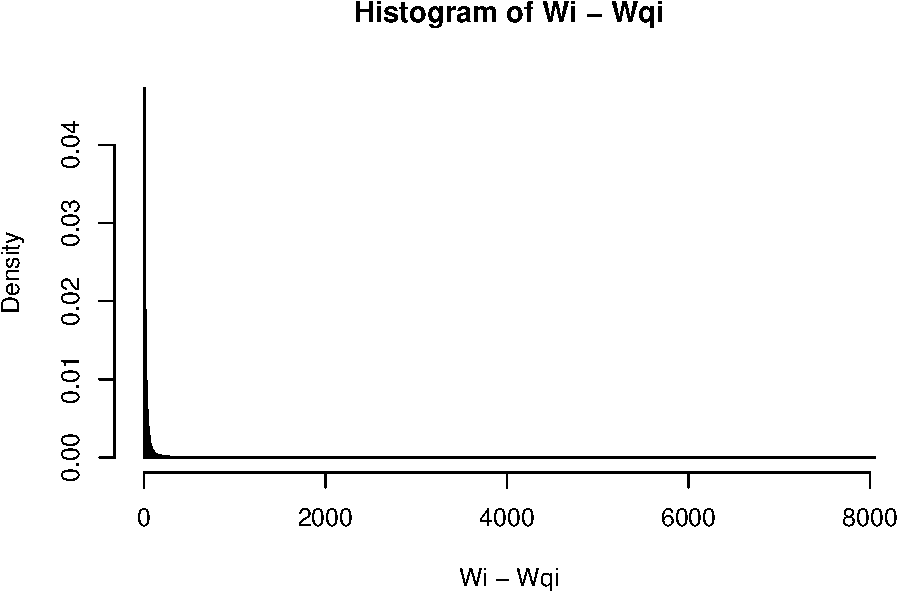
\includegraphics[width=0.5\linewidth]{003_files/figure-latex/unnamed-chunk-6-1} \end{center}

We can clearly observe that the service times follow a heavy-tailed
distribution, as more than 75\% of the histogram bins have few samples
and they are all consecutively placed until the end of it.

The mean and sample variance of the services times are the following:

\begin{enumerate}
\def\labelenumi{\arabic{enumi}.}
\tightlist
\item
  Mean of the service times: \(W_{s_{avg}}\)=30.4132959
\item
  Standard deviation of the service times: \(W_{s_{std}}\)=77.5293542
\item
  Coeficient of variation: \(C_{x}={ \sigma_{x} \over E[x] }\)=2.5491928
\end{enumerate}

The Theoretical values for a Lognormal with \(\mu\)=2.4070657 and
\(\sigma\)=1.4286 are the follwing:

\begin{enumerate}
\def\labelenumi{\arabic{enumi}.}
\tightlist
\item
  Mean of the service times: \(E[x]\)=30.8
\item
  Standard deviation of the service times: \(sqrt{Var[x]}\)=79.7090561
\item
  Coeficient of variation: \(C_{x}={ \sigma_{x} \over E[x] }\)=2.5879564
\end{enumerate}

We observe that the sample statistics are close to the theoretical
values. Our simulation can be considered to be correct.

\subsection{\texorpdfstring{Allen Cuneen's aproximation formula for
\(W_{q}\) and
\(L_{q}\)}{Allen Cuneen's aproximation formula for W\_\{q\} and L\_\{q\}}}\label{allen-cuneens-aproximation-formula-for-w_q-and-l_q}

For each loading factor \(\rho\), we derive the required \(\mu\) value
for the Lognormal distribution:

\begin{itemize}
\tightlist
\item
  \(s = 1\), \(\lambda = { 1 \over E[\tau] }\) ,
  \(\mu = {1 \over E[x]}\)
\item
  \(E[x] = m \cdot e^{\sigma^{2} \over 2} = e^{\mu + {\sigma^{2} \over 2} }\)
\item
  \(\rho = { \lambda \over {s\mu}} = { E[x] \over E[\tau] } = e^{\mu} \cdot { e^{\sigma^{2} \over 2} \over E[x] } \Rightarrow \mu = ln \left( { \rho \over e^{ \sigma^{2} \over 2 } } \cdot E[\tau] \right)\)
\end{itemize}

We use the Allen Cuneen's approximation formula for \(L_{q}\):

\begin{itemize}
\tightlist
\item
  \(L_{q} \approx L_{q_{M/M/1}} \cdot \left( C_{\tau}^{2} + C_{x}^{2} \over 2 \right)\)
\item
  with: \(C_{x} = \sqrt{ \omega - 1} = \sqrt{ e^{\sigma^{2}} - 1}\) and
  \(C_{\tau} = { \sigma_{\tau} \over E[\tau] }\)
\item
  and derive \(W_{q} = { L_{q} \over \lambda }\)
\end{itemize}

Using the Allen Cuneen's approximation formula, we can compute the
\(W_{q}\) and \(L_{q}\) for each loading factor:

\begin{longtable}[]{@{}llll@{}}
\toprule
\(\rho\) & \(\mu\) & \(W_{q}\) & \(L_{q}\)\tabularnewline
\midrule
\endhead
0.4 & 2.4070657 & 69.1507968 & 0.8980623\tabularnewline
0.7 & 2.9666815 & 423.5486306 & 5.5006316\tabularnewline
0.85 & 3.1608375 & 1249.0362678 & 16.2212502\tabularnewline
0.925 & 3.2453949 & 2958.3575269 & 38.4202276\tabularnewline
\bottomrule
\end{longtable}

\subsection{Simulation}\label{simulation}

First, for each \(\rho\), we're going to calculate what is the amount of
clients needed to get in the steady state of the waiting system.

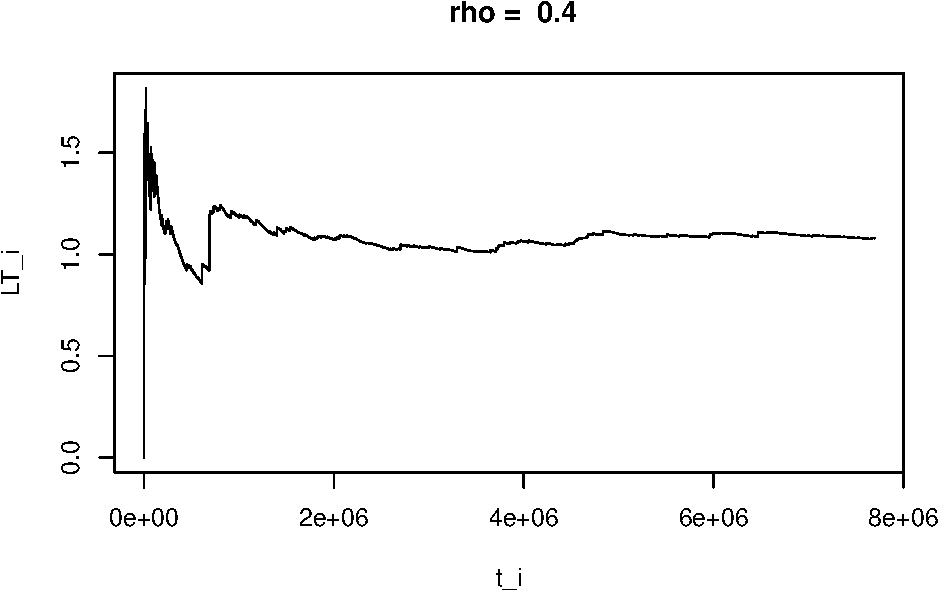
\includegraphics{003_files/figure-latex/unnamed-chunk-10-1.pdf}
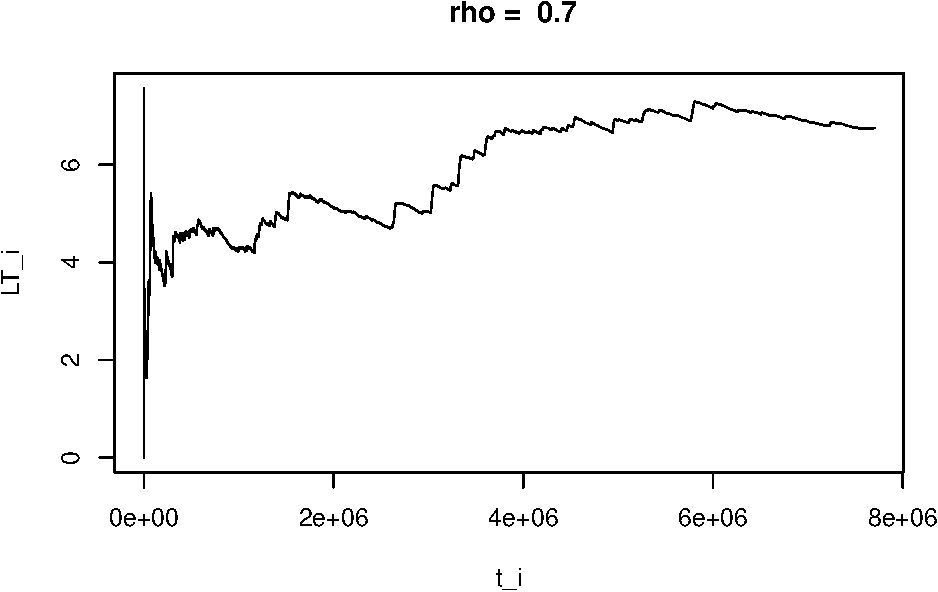
\includegraphics{003_files/figure-latex/unnamed-chunk-10-2.pdf}
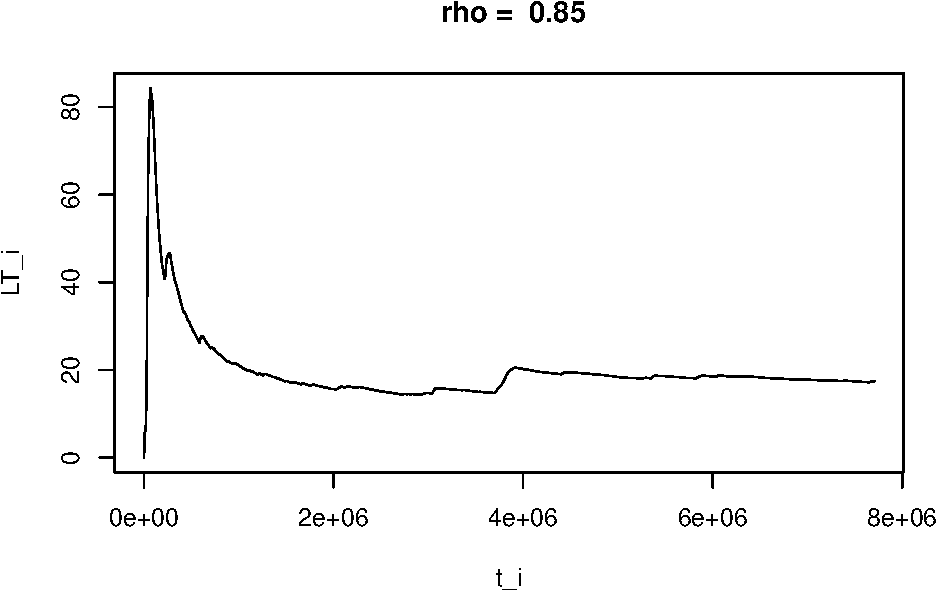
\includegraphics{003_files/figure-latex/unnamed-chunk-10-3.pdf}
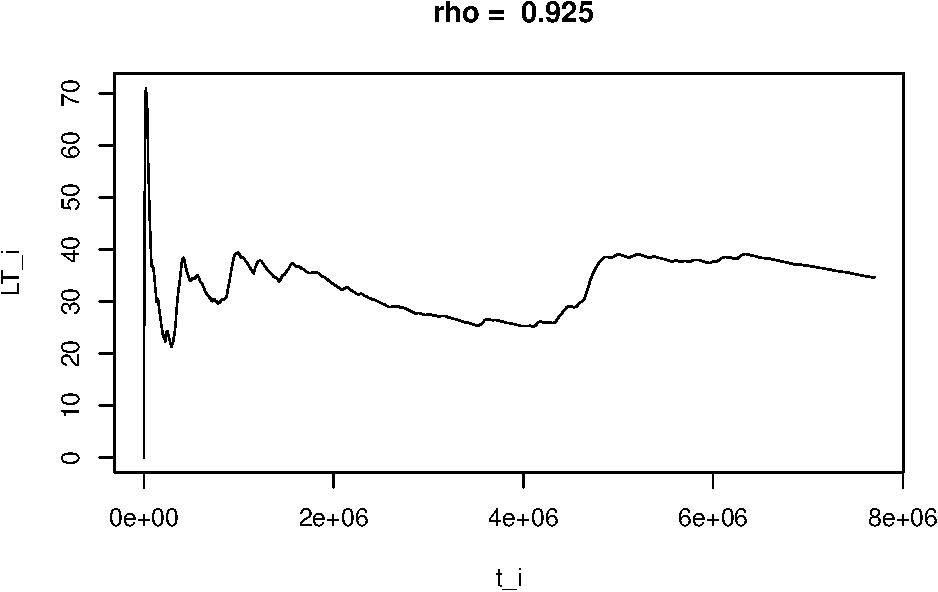
\includegraphics{003_files/figure-latex/unnamed-chunk-10-4.pdf}

We observe that, apart from the simulation with loading factor 0.4, the
other simulations have not attained the steady state.

If we repeat the simulations with a number of clients between 200000 and
500000, the steady state is attained with all loading factors. We have
not tested more than 500000 clients.

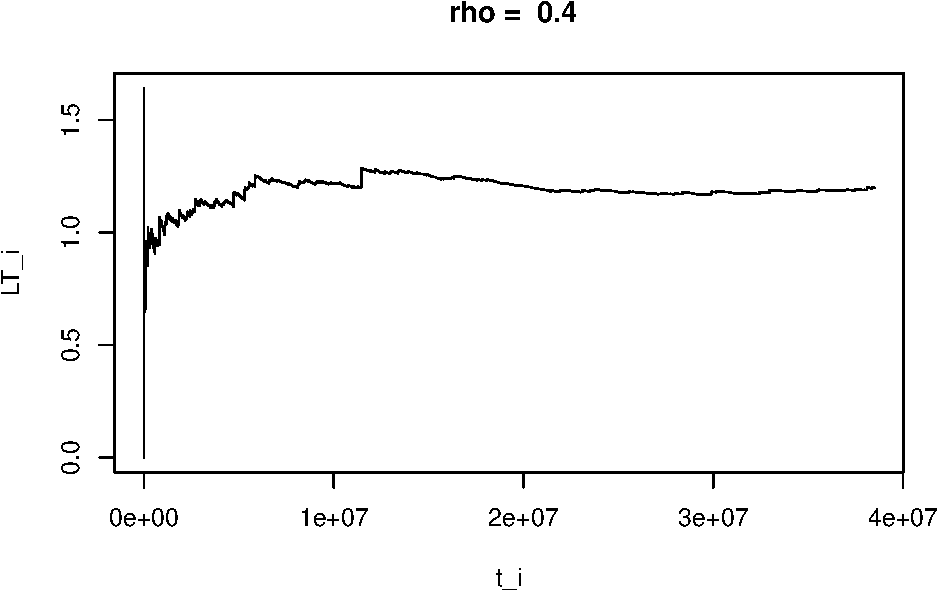
\includegraphics{003_files/figure-latex/unnamed-chunk-11-1.pdf}
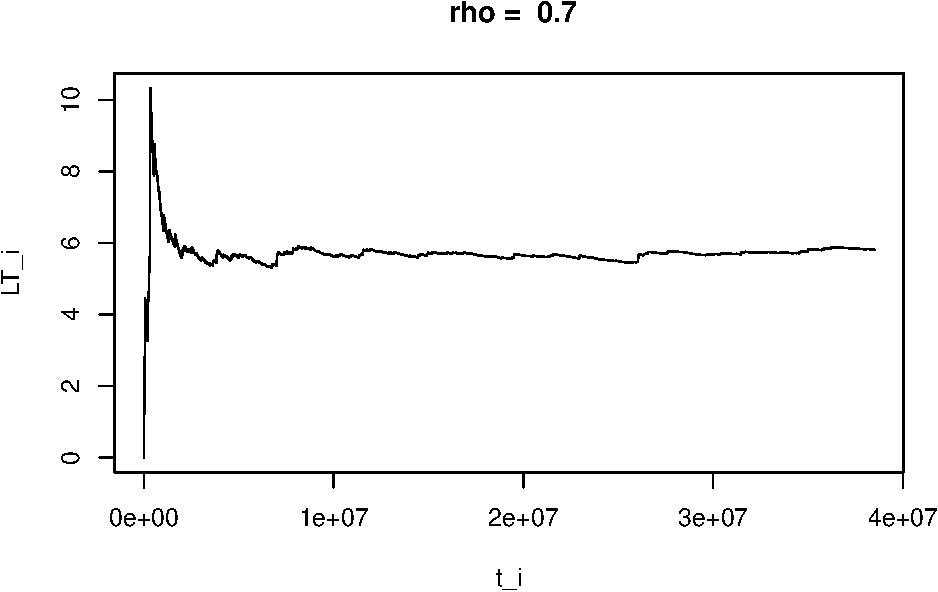
\includegraphics{003_files/figure-latex/unnamed-chunk-11-2.pdf}
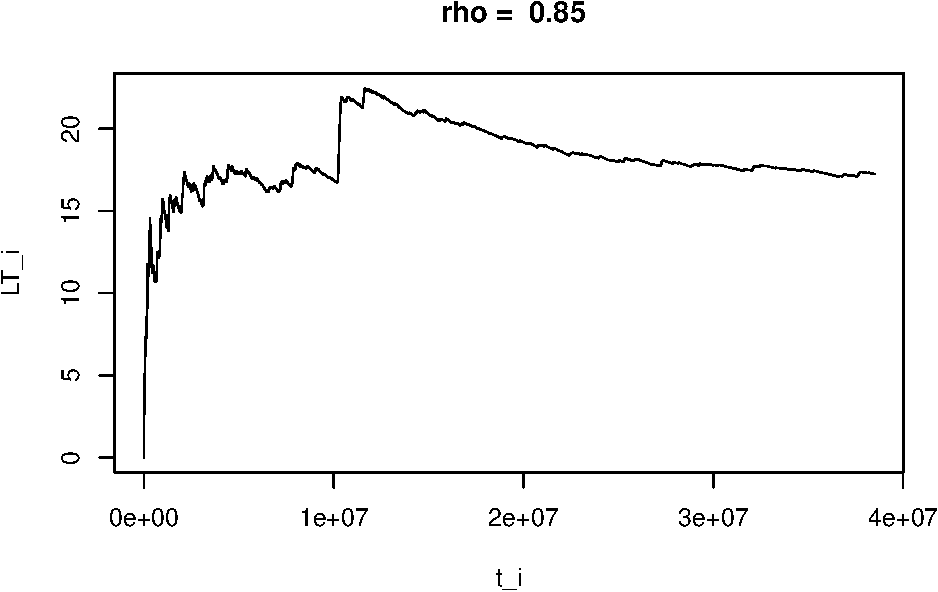
\includegraphics{003_files/figure-latex/unnamed-chunk-11-3.pdf}
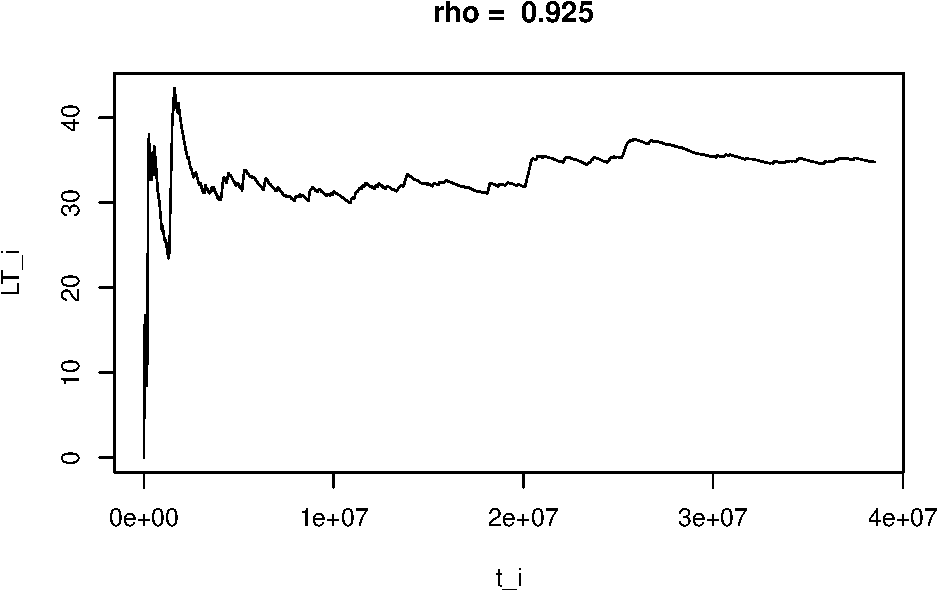
\includegraphics{003_files/figure-latex/unnamed-chunk-11-4.pdf}

\subsubsection{\texorpdfstring{Loading factor \(\rho\) =
0.4}{Loading factor \textbackslash{}rho = 0.4}}\label{loading-factor-rho-0.4}

We generate 10 simulations with 100000 clients, each with a different
seed. For each simulation, we check if the steady state is attained
without any abrupt increase or decrease in the value of the average
occupancy. In case there's any abrupt increase or decrease, we change
the seed. If for many seeds, this phenomena is still happening, we
increase the number of clients.

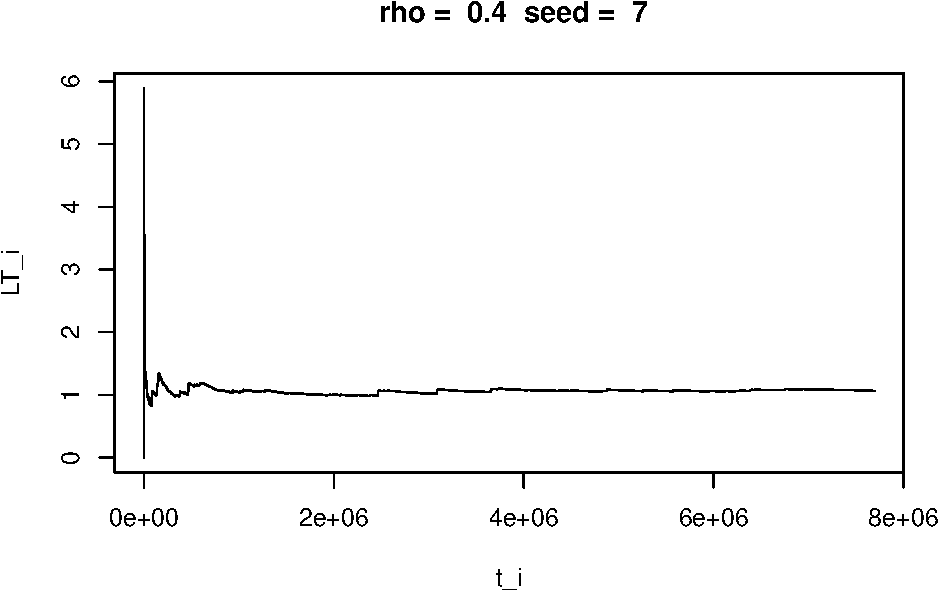
\includegraphics{003_files/figure-latex/unnamed-chunk-13-1.pdf}
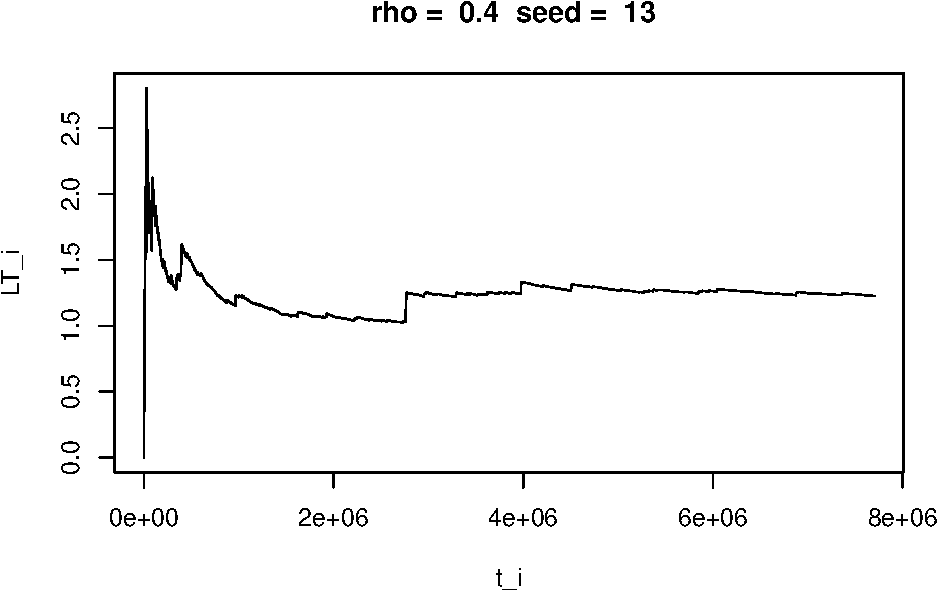
\includegraphics{003_files/figure-latex/unnamed-chunk-13-2.pdf}
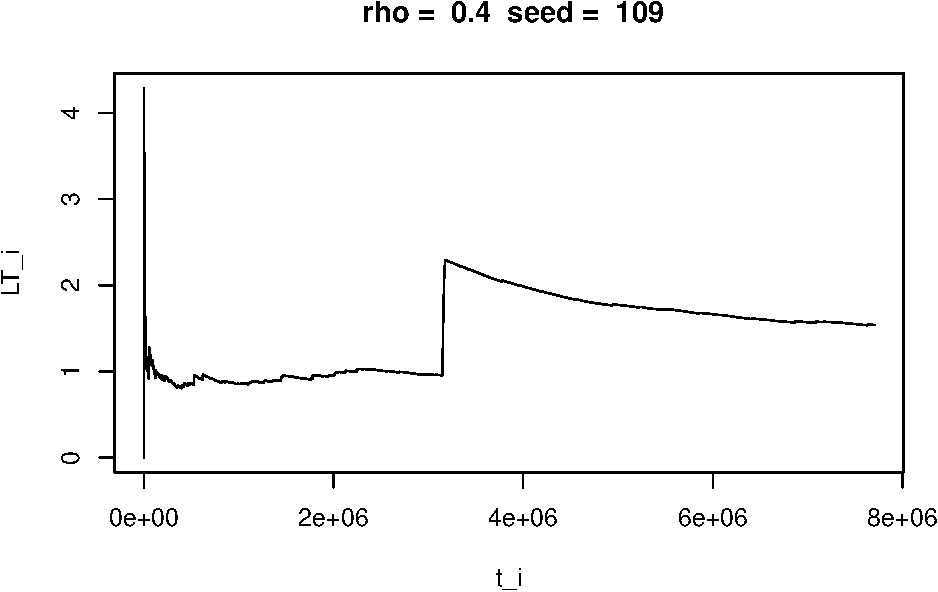
\includegraphics{003_files/figure-latex/unnamed-chunk-13-3.pdf}
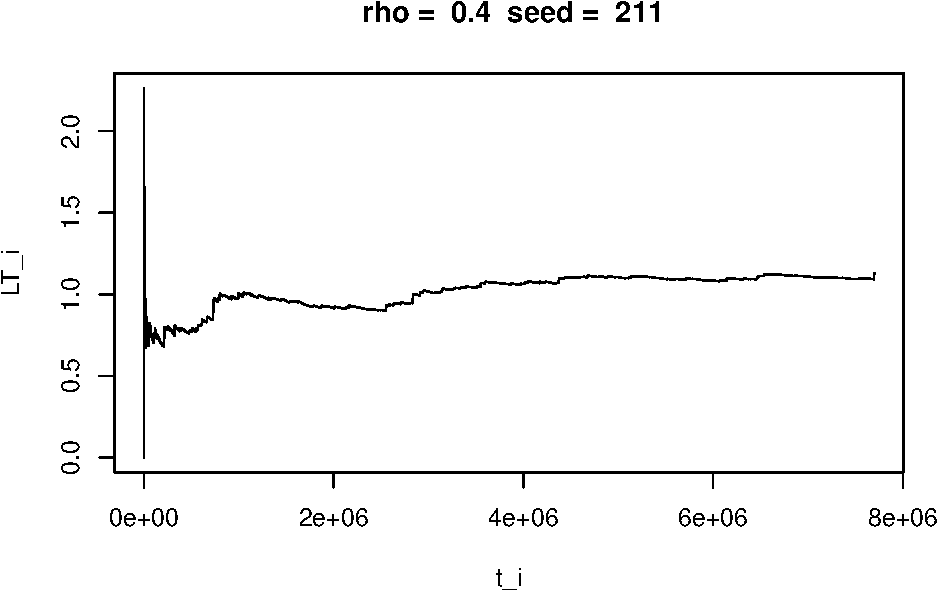
\includegraphics{003_files/figure-latex/unnamed-chunk-13-4.pdf}
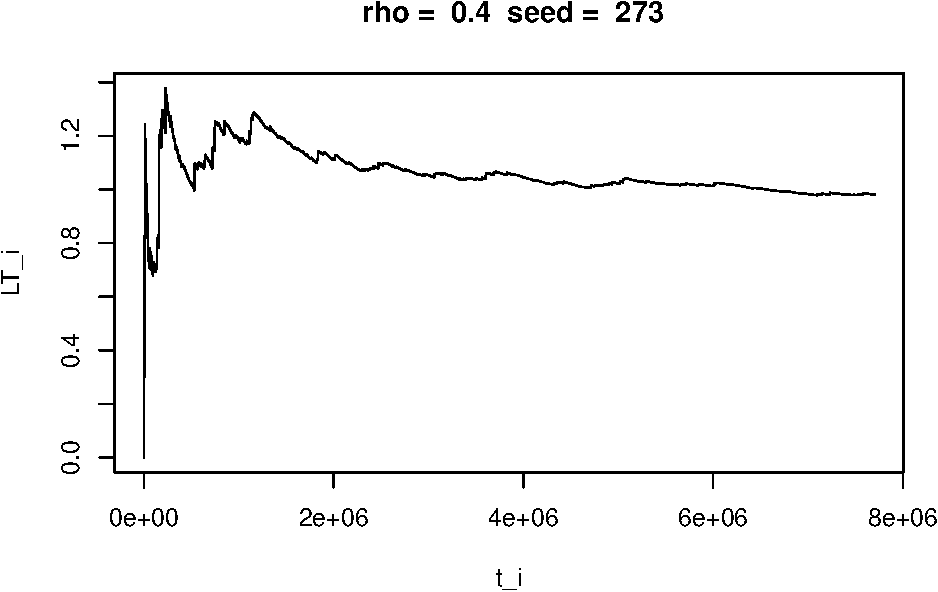
\includegraphics{003_files/figure-latex/unnamed-chunk-13-5.pdf}
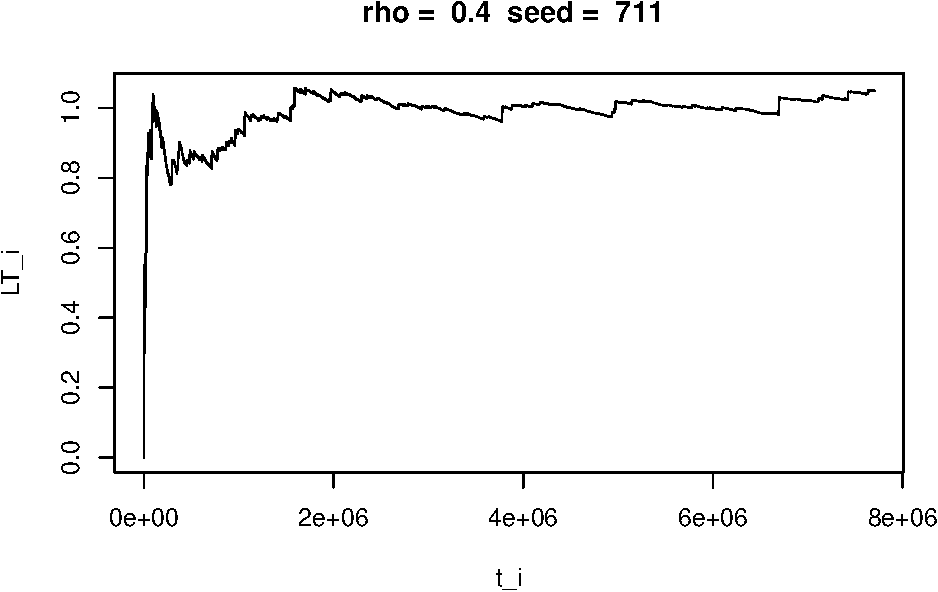
\includegraphics{003_files/figure-latex/unnamed-chunk-13-6.pdf}
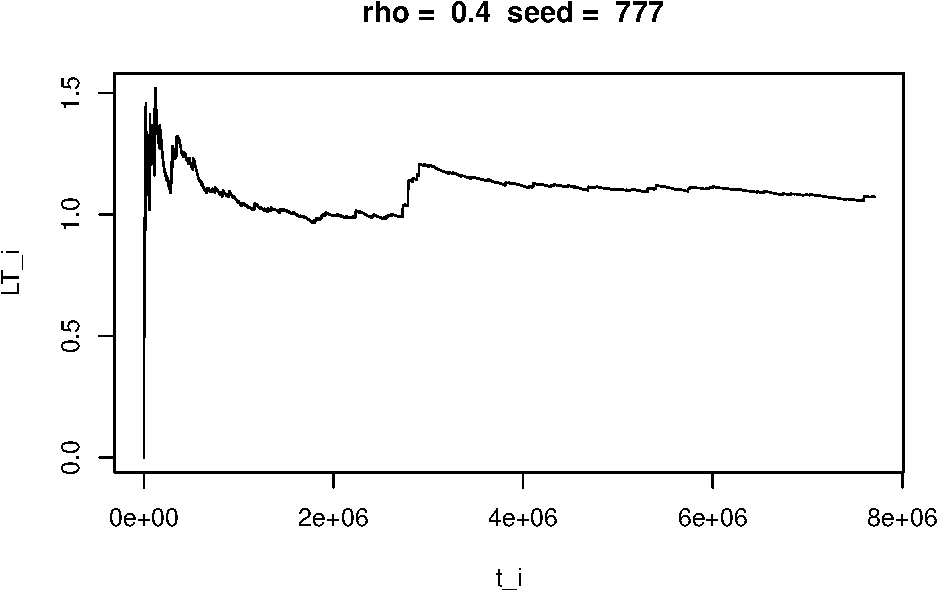
\includegraphics{003_files/figure-latex/unnamed-chunk-13-7.pdf}
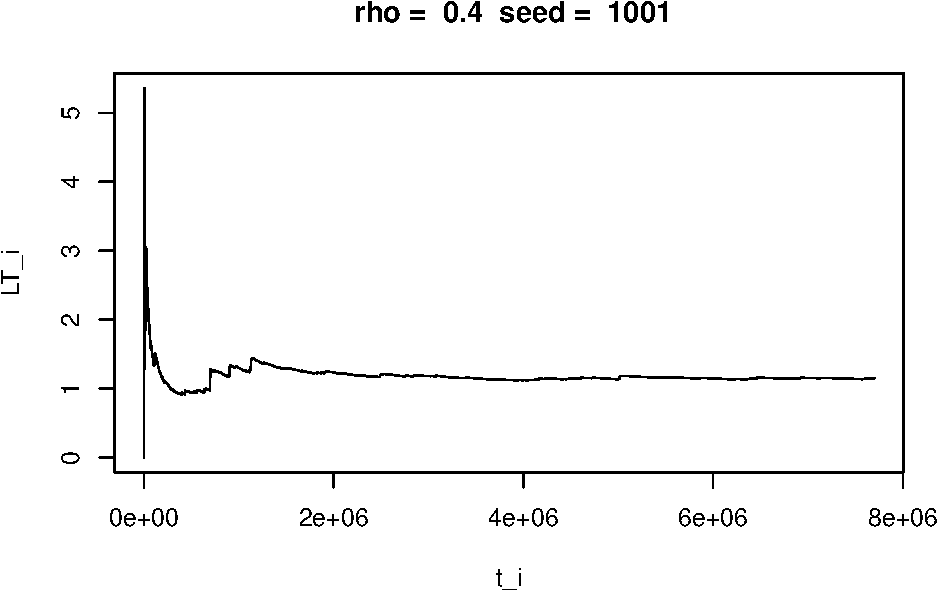
\includegraphics{003_files/figure-latex/unnamed-chunk-13-8.pdf}
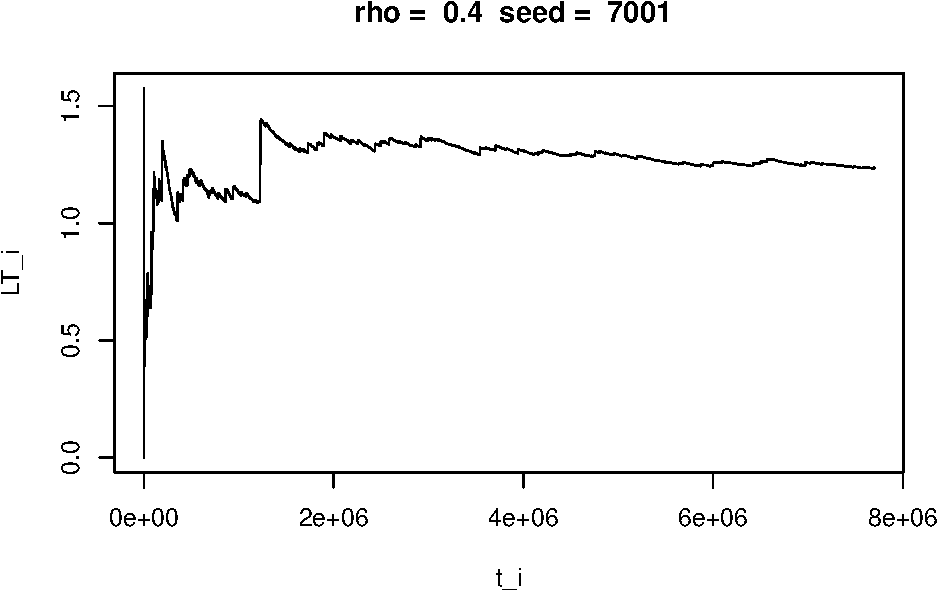
\includegraphics{003_files/figure-latex/unnamed-chunk-13-9.pdf}
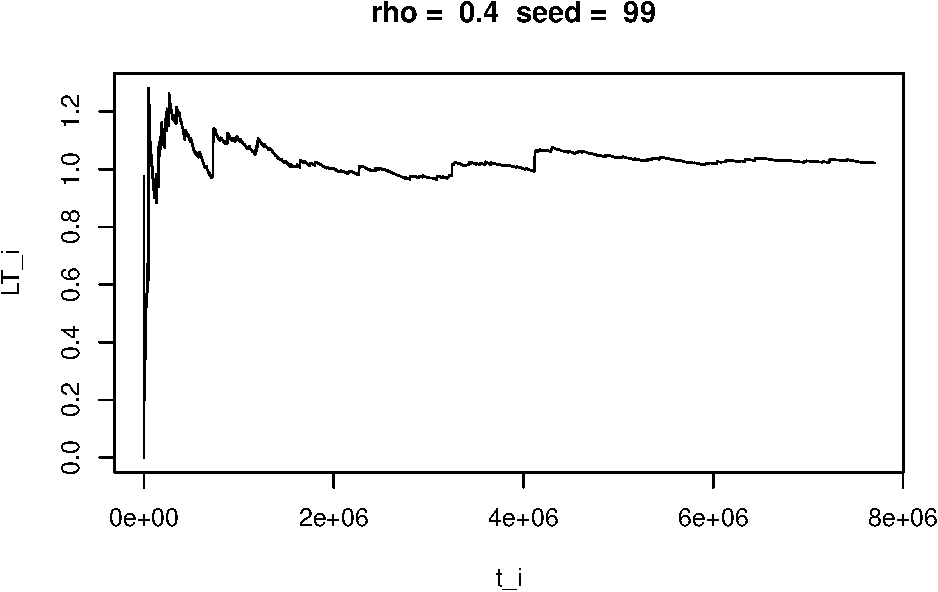
\includegraphics{003_files/figure-latex/unnamed-chunk-13-10.pdf}

We observe that for the seeds 10101, 1078, 960 and 51, there's an abrupt
change in the average occupancy. We change those seeds and redo the
simulation.

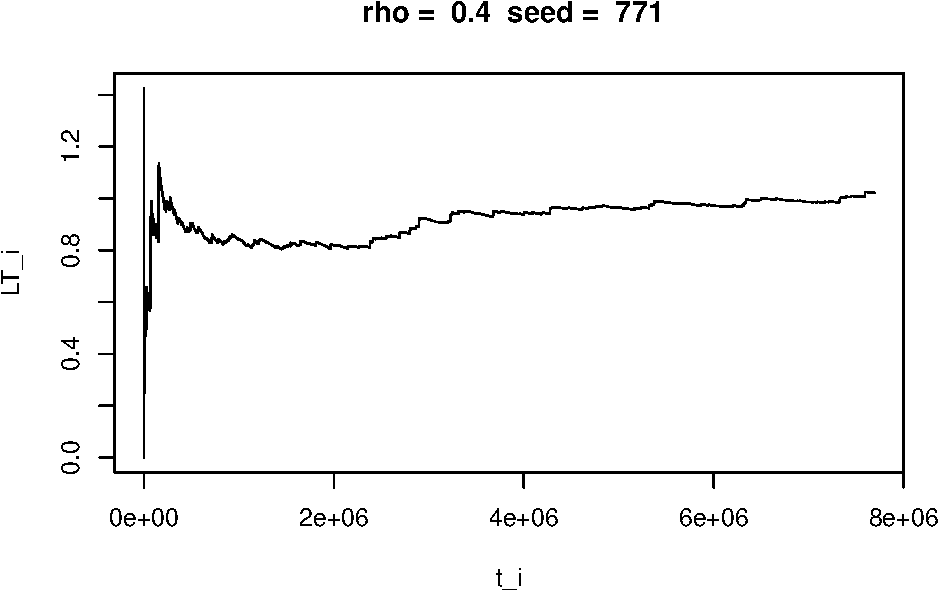
\includegraphics{003_files/figure-latex/unnamed-chunk-14-1.pdf}
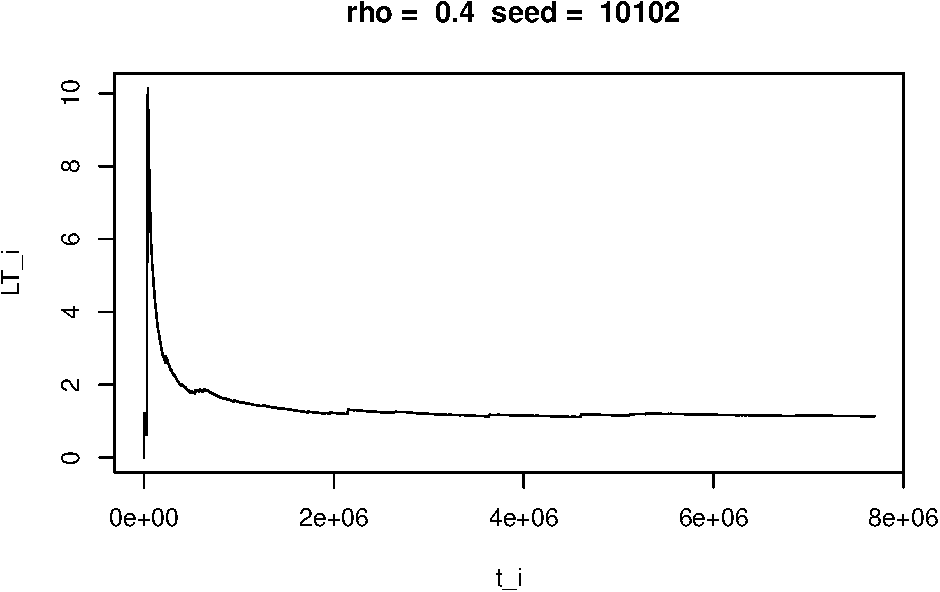
\includegraphics{003_files/figure-latex/unnamed-chunk-14-2.pdf}
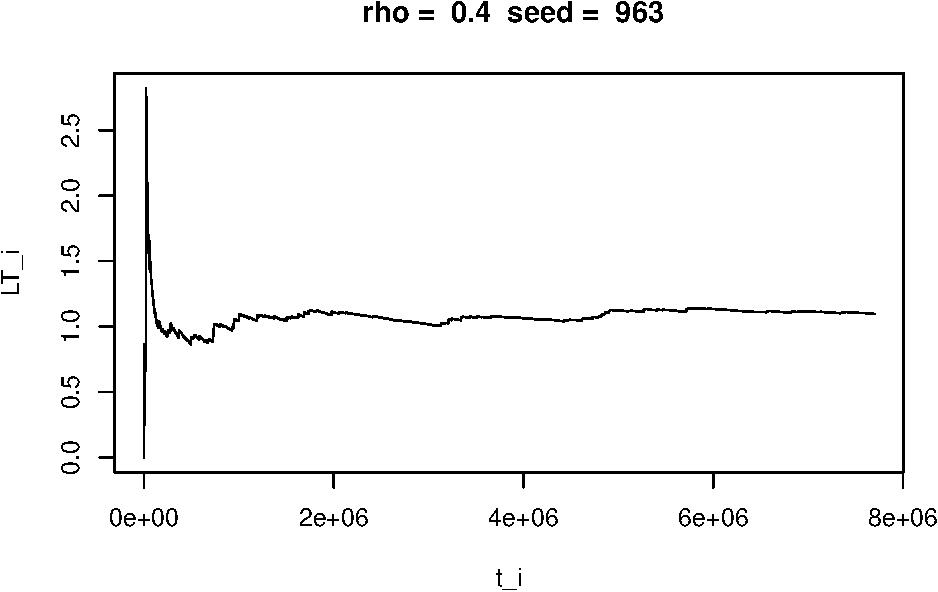
\includegraphics{003_files/figure-latex/unnamed-chunk-14-3.pdf}
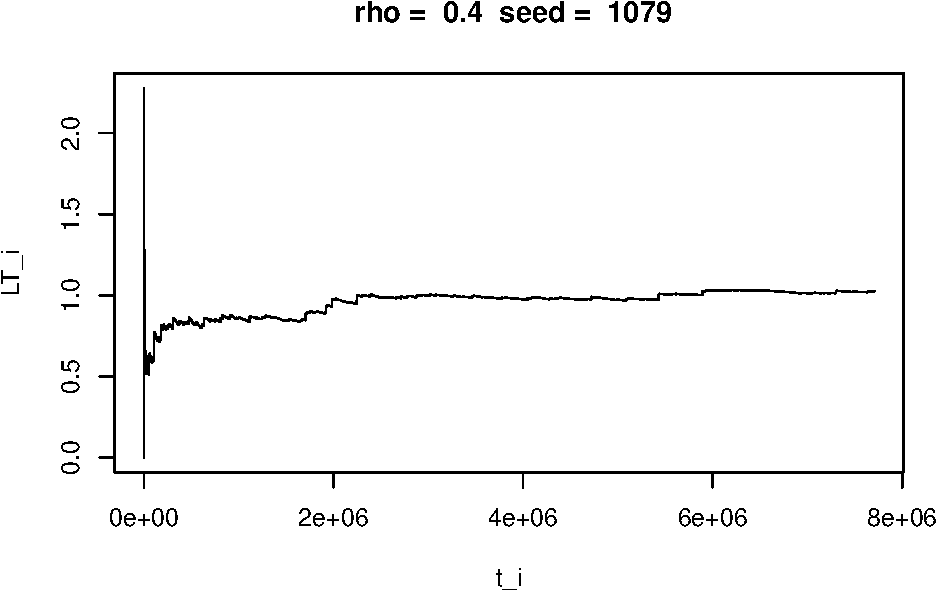
\includegraphics{003_files/figure-latex/unnamed-chunk-14-4.pdf}
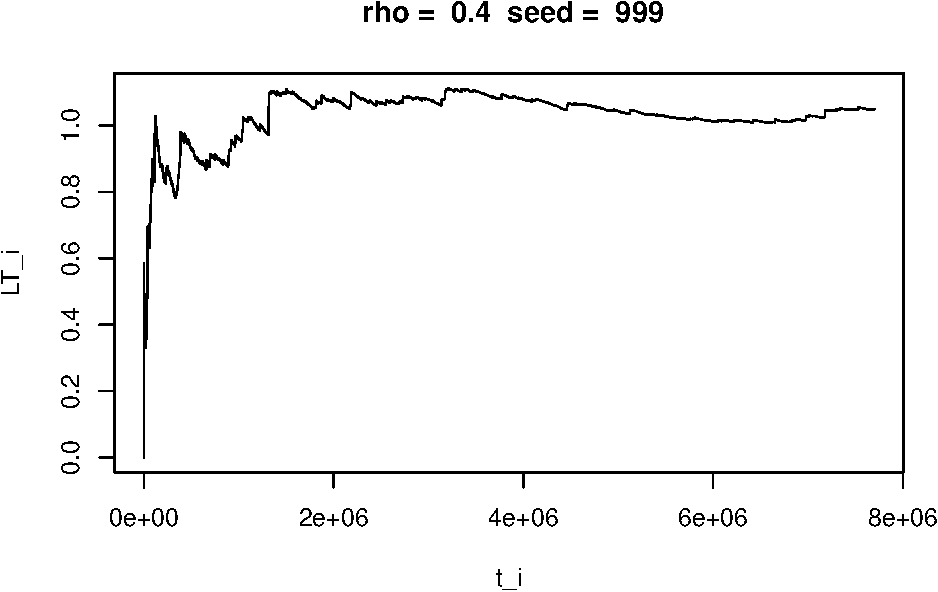
\includegraphics{003_files/figure-latex/unnamed-chunk-14-5.pdf}
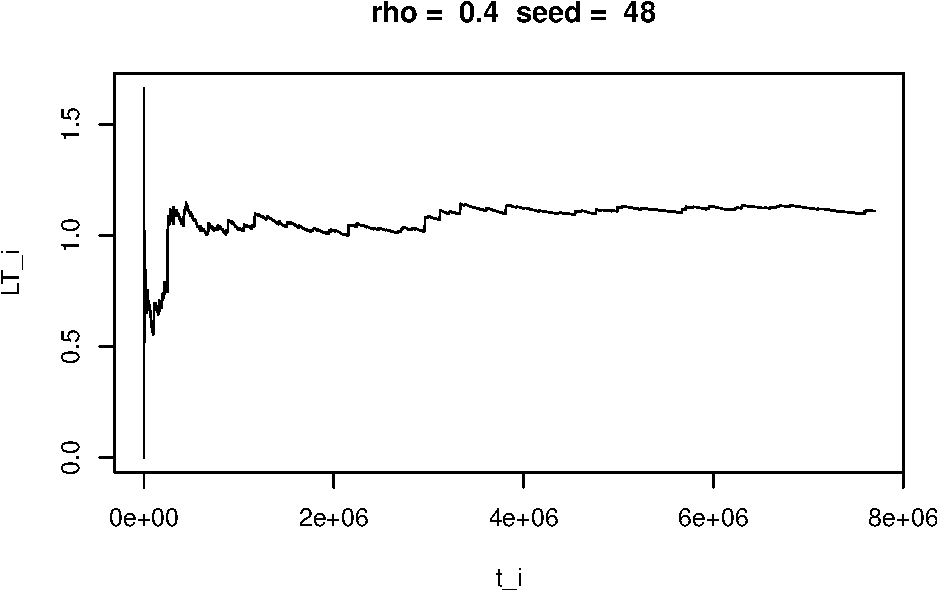
\includegraphics{003_files/figure-latex/unnamed-chunk-14-6.pdf}
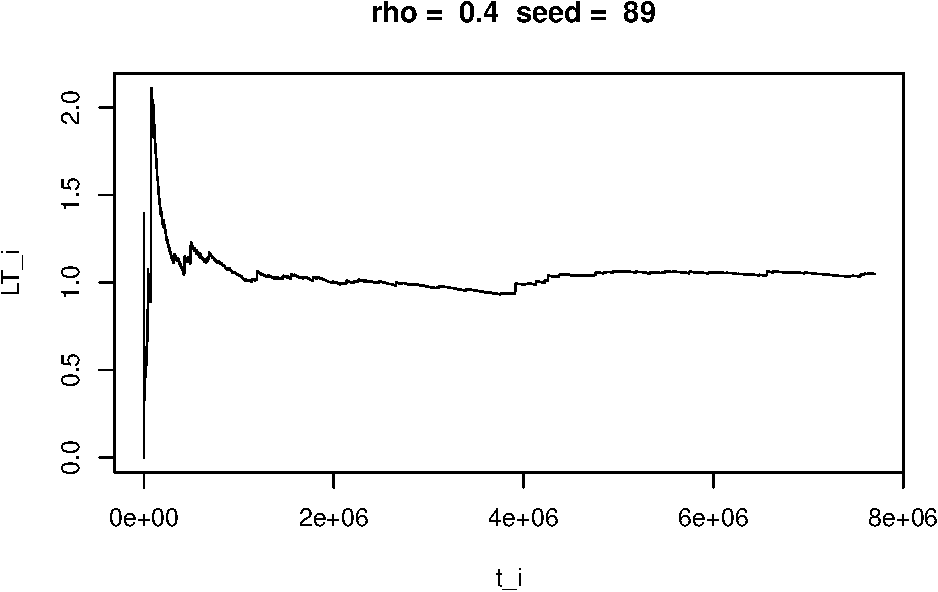
\includegraphics{003_files/figure-latex/unnamed-chunk-14-7.pdf}
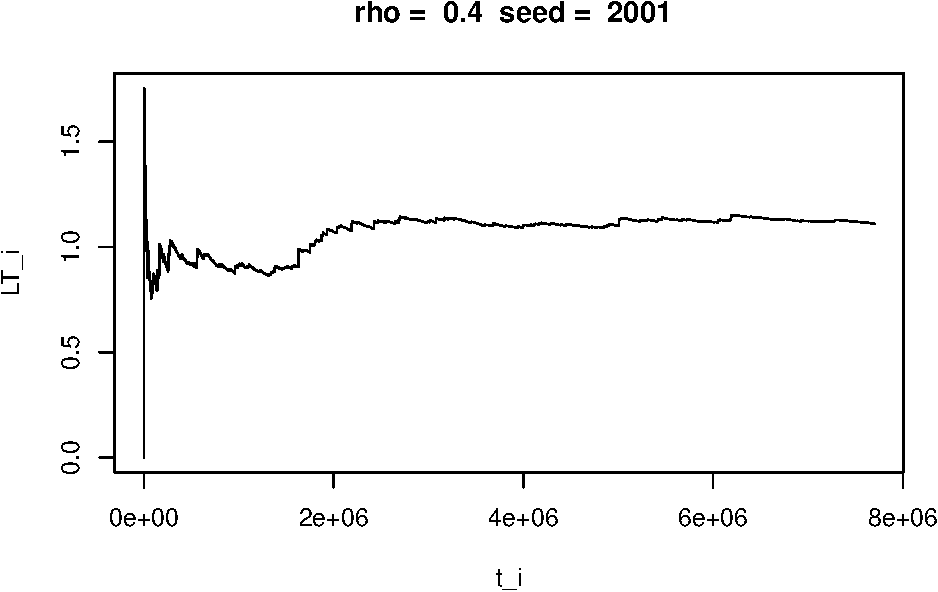
\includegraphics{003_files/figure-latex/unnamed-chunk-14-8.pdf}
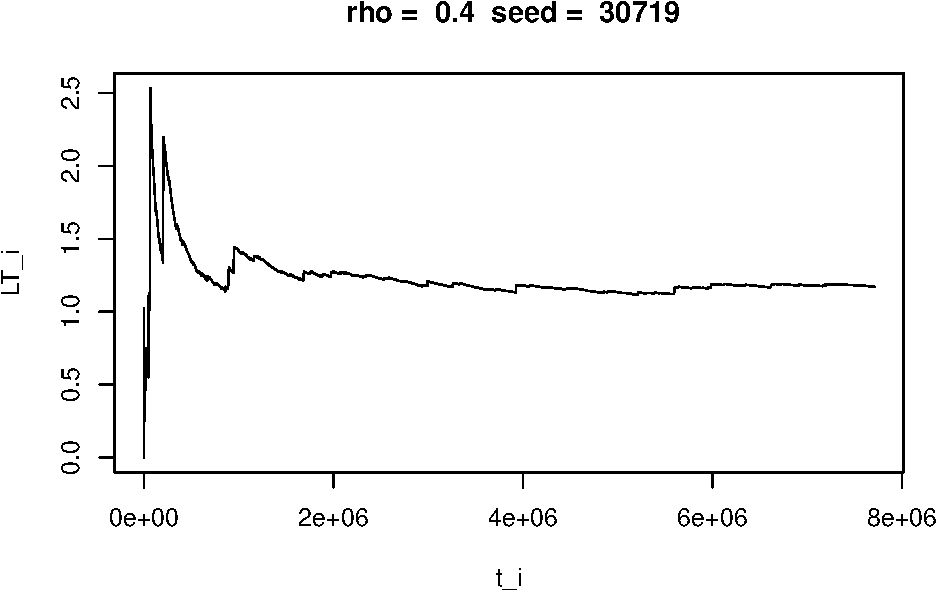
\includegraphics{003_files/figure-latex/unnamed-chunk-14-9.pdf}
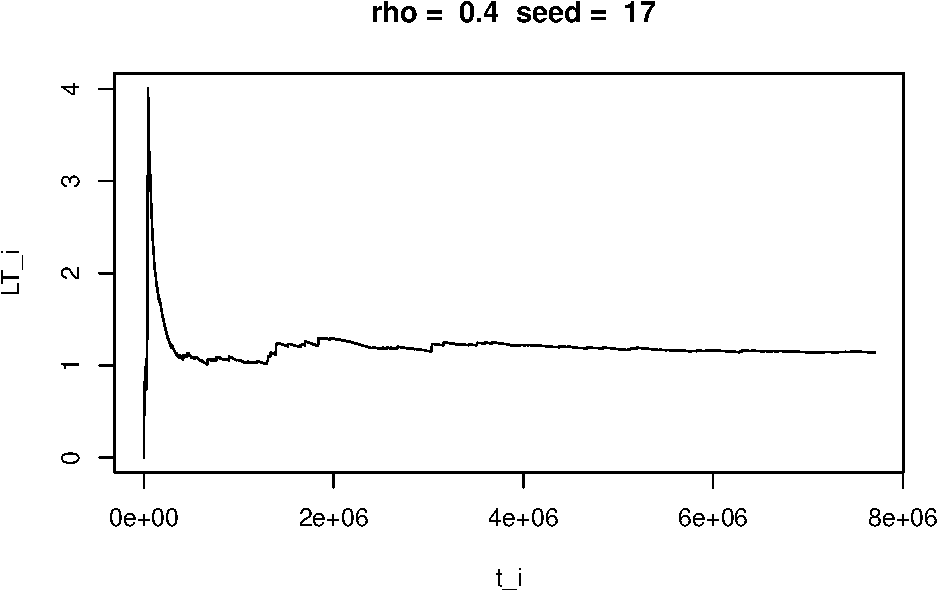
\includegraphics{003_files/figure-latex/unnamed-chunk-14-10.pdf}

We changed a total of 4 out of 10 seeds.

We now compute the confidence interval for \(L_{q}\) and \(W_{q}\). We
will use a t-Student distribution with critical value 1 - 0.95 and 9
degrees of freedom to compute a 95\% confidence interval.

\begin{itemize}
\tightlist
\item
  \(L_{q_{1}},L_{q_{2}},...,L_{q_{10}}\), and
  \(\overline{L}_{q} = {1 \over n}\sum_{i=1}^{n}L_{q_{i}}\)
\item
  \(S_{L_{q}}^{2} = {1 \over n - 1} \sum_{i=1}^{n} ( L_{q_{i}} - \overline{L}_{q} )^{2}\)
\end{itemize}

To get:
\[C.I.(L_{q}) =   \overline{L}_{q} \pm t_{1 - \alpha, n - 1} \cdot \sqrt{S_{L_{q}}^{2} \over n}\]

And then:

\begin{itemize}
\tightlist
\item
  \(W_{q_{1}},W_{q_{2}},...,W_{q_{10}}\), and
  \(\overline{W}_{q} = {1 \over n}\sum_{i=1}^{n}W_{q_{i}}\)
\item
  \(S_{W_{q}}^{2} = {1 \over n - 1} \sum_{i=1}^{n} ( W_{q_{i}} - \overline{W}_{q} )^{2}\)
\end{itemize}

to get:
\[ C.I.(W_{q}) =   \overline{W}_{q} \pm t_{1 - \alpha, n - 1} \cdot \sqrt{S_{W_{q}}^{2} \over n}\]

The computations produce the followings confidence intervals for the
average queue length and waiting time:

\begin{longtable}[]{@{}llllll@{}}
\toprule
\(\rho\) & -C.I \(W_{q}\) & +C.I \(W_{q}\) & -C.I \(L_{q}\) & +C.I
\(L_{q}\) &\tabularnewline
\midrule
\endhead
0.4 & 0.6629266 & 0.7216626 & 51.0353731 & 55.5687961\tabularnewline
\bottomrule
\end{longtable}

\subsubsection{\texorpdfstring{Loading factor \(\rho\) =
0.7}{Loading factor \textbackslash{}rho = 0.7}}\label{loading-factor-rho-0.7}

We follow the same procedure to generate 10 simulations with 100000
clients, as we did for the previous \(\rho=\), correcting any invalid
seeds for the ramdom number generator. The result is that we need to
increase the number of clients to 500000 to be sure that the system has
arribed to the steady state.

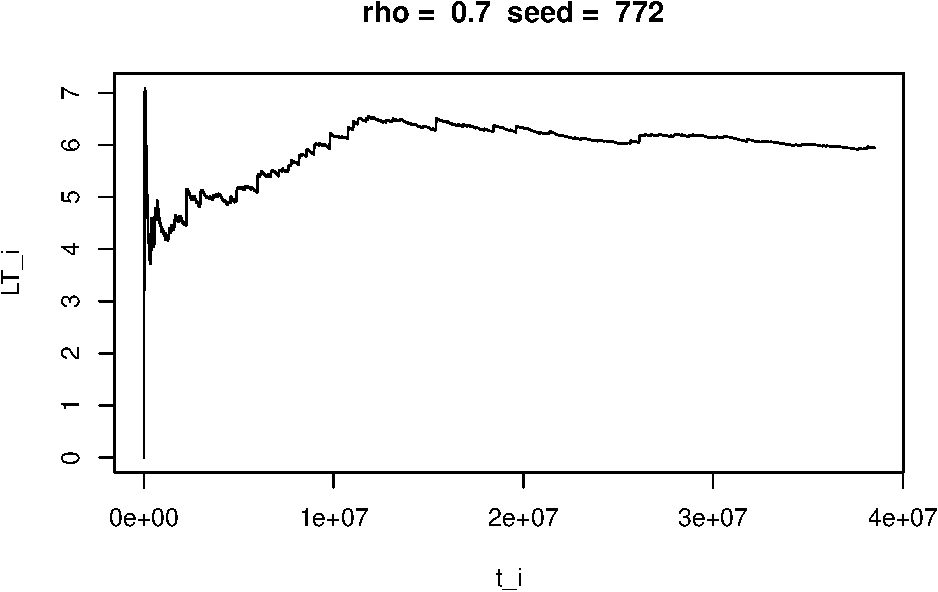
\includegraphics{003_files/figure-latex/unnamed-chunk-17-1.pdf}
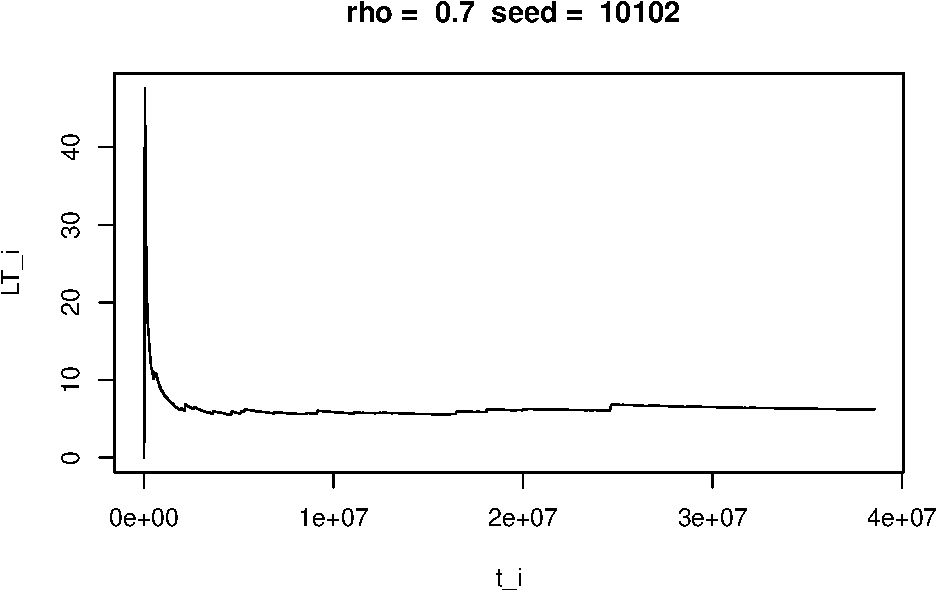
\includegraphics{003_files/figure-latex/unnamed-chunk-17-2.pdf}
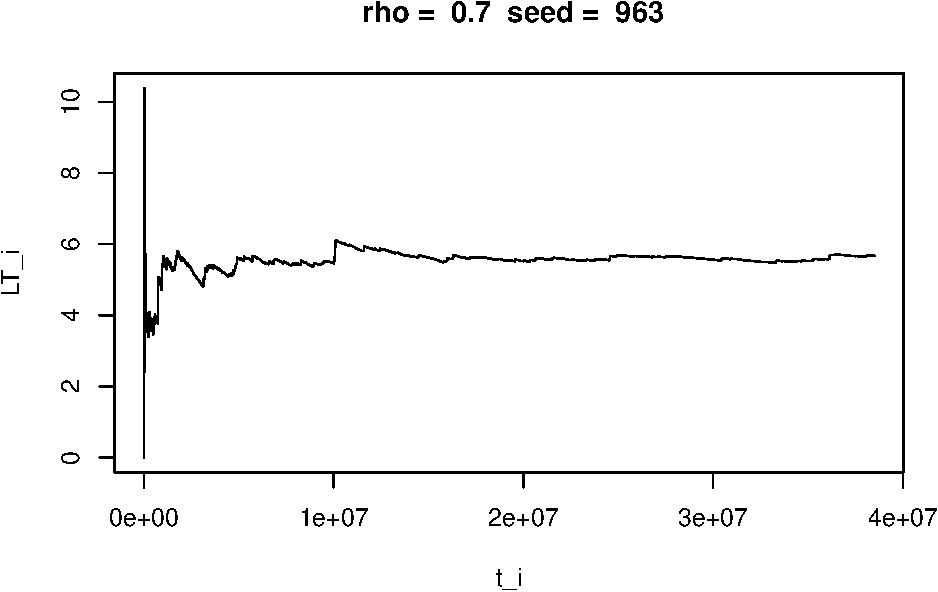
\includegraphics{003_files/figure-latex/unnamed-chunk-17-3.pdf}
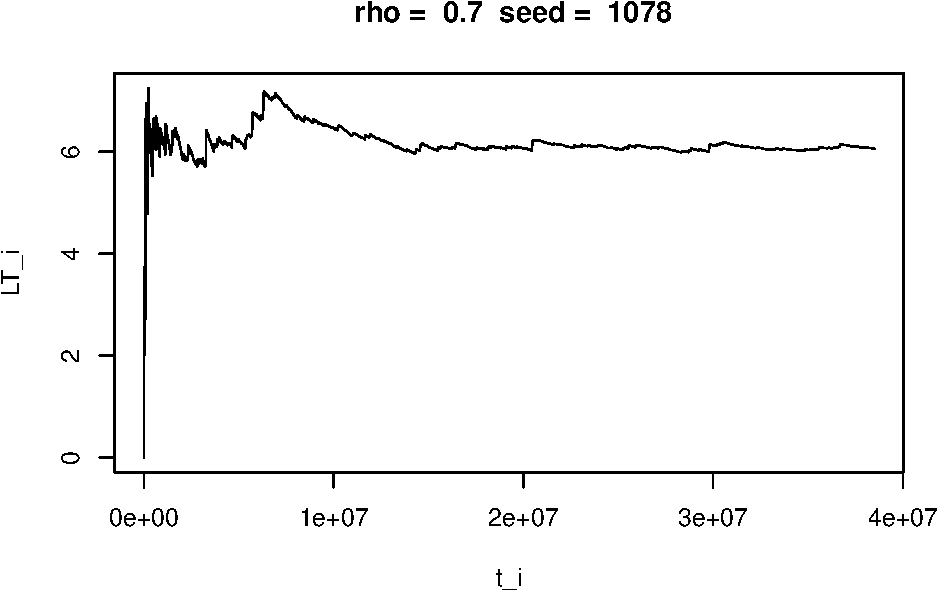
\includegraphics{003_files/figure-latex/unnamed-chunk-17-4.pdf}
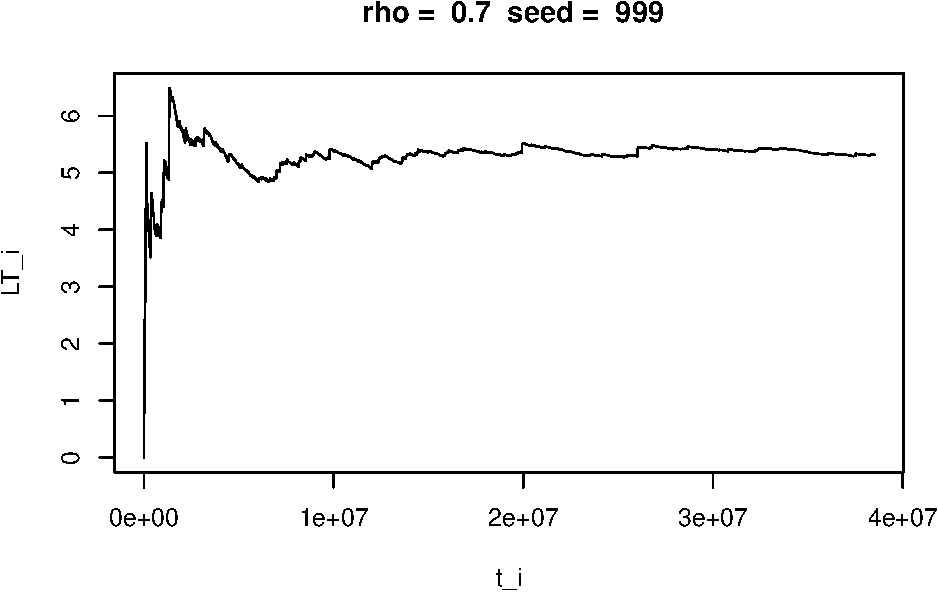
\includegraphics{003_files/figure-latex/unnamed-chunk-17-5.pdf}
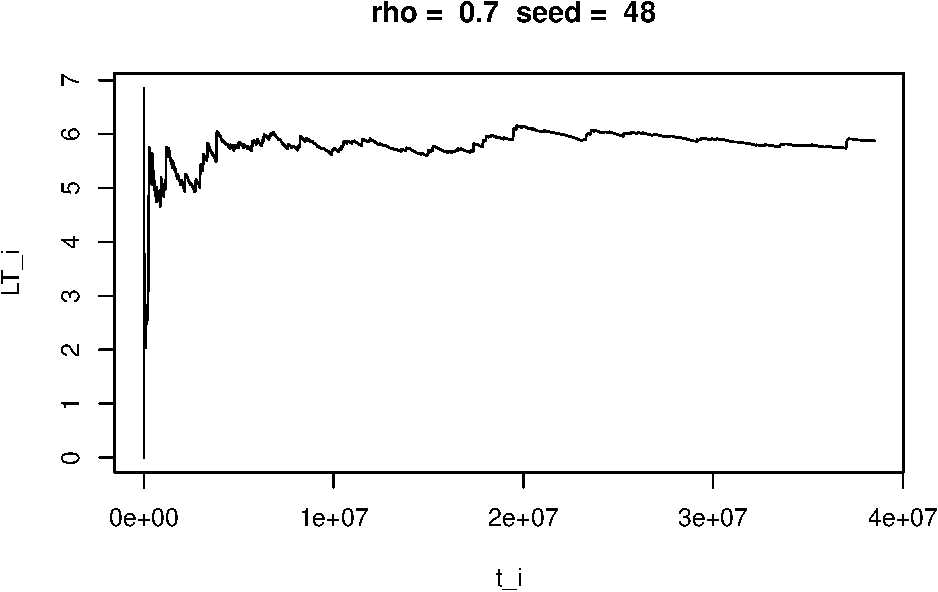
\includegraphics{003_files/figure-latex/unnamed-chunk-17-6.pdf}
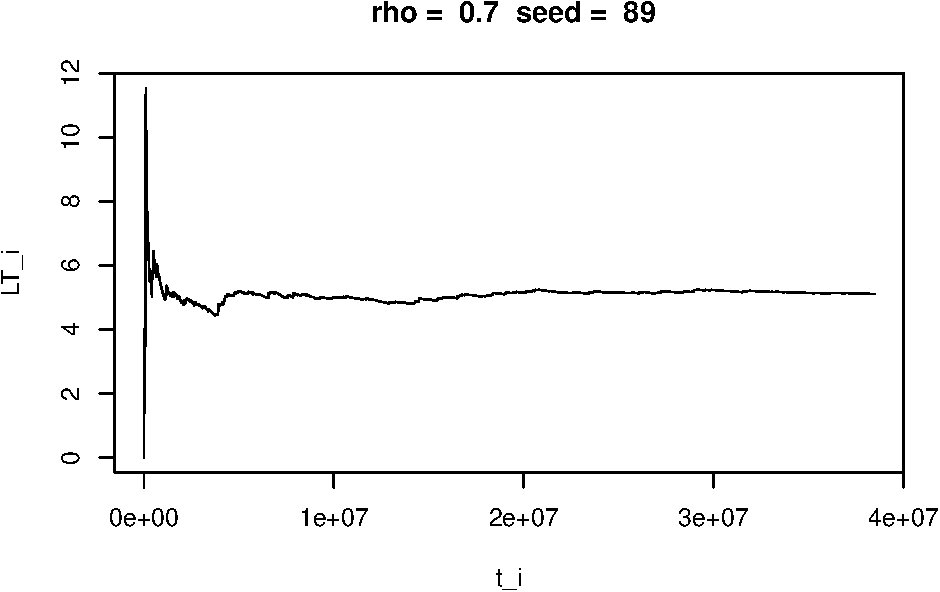
\includegraphics{003_files/figure-latex/unnamed-chunk-17-7.pdf}
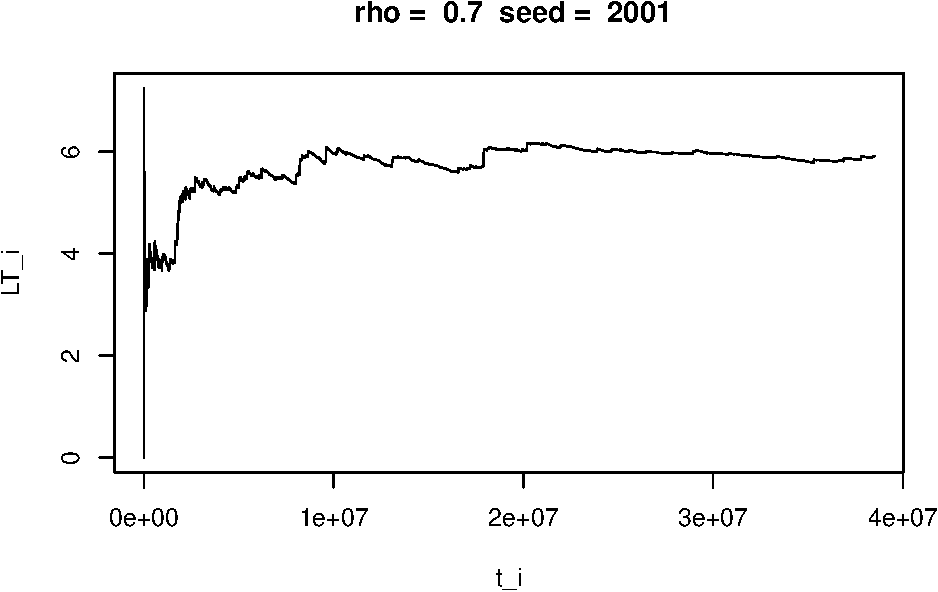
\includegraphics{003_files/figure-latex/unnamed-chunk-17-8.pdf}
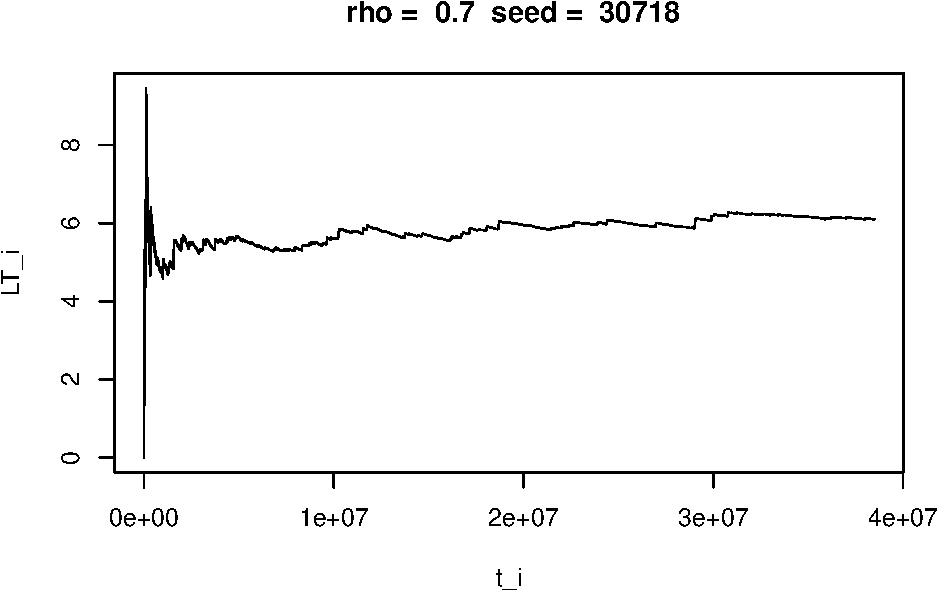
\includegraphics{003_files/figure-latex/unnamed-chunk-17-9.pdf}
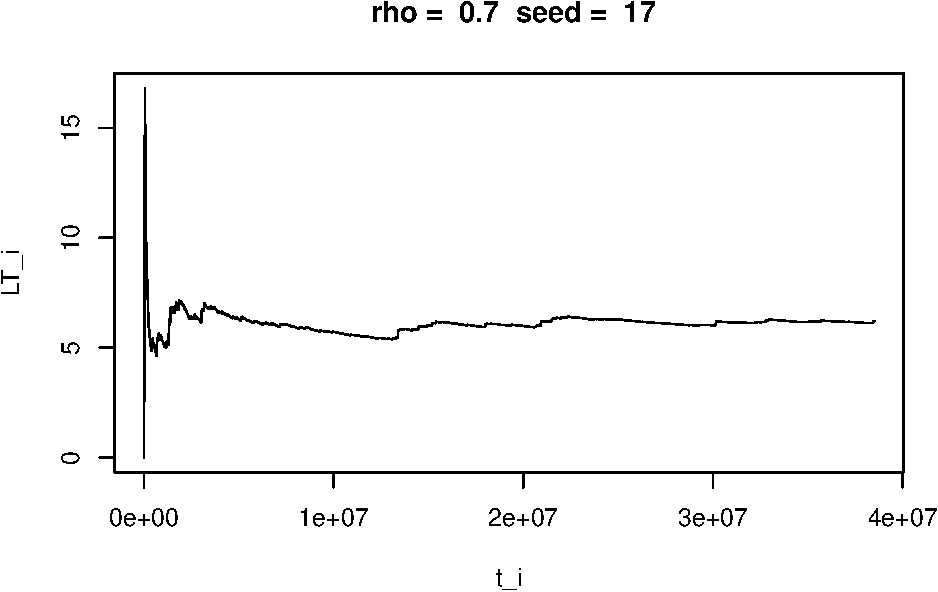
\includegraphics{003_files/figure-latex/unnamed-chunk-17-10.pdf}

We now compute the confidence interval for \(L_{q}\) and \(W_{q}\) using
the same procedure we detailed for \(\rho =\) 0.7. The computations
produce the followings confidence intervals for the average queue length
and waiting time:

\begin{longtable}[]{@{}llllll@{}}
\toprule
\(\rho\) & -C.I \(W_{q}\) & +C.I \(W_{q}\) & -C.I \(L_{q}\) & +C.I
\(L_{q}\) &\tabularnewline
\midrule
\endhead
0.7 & 4.9266678 & 5.3560657 & 379.3389492 & 412.4915102\tabularnewline
\bottomrule
\end{longtable}

\subsubsection{\texorpdfstring{Loading factor \(\rho\) =
0.85}{Loading factor \textbackslash{}rho = 0.85}}\label{loading-factor-rho-0.85}

We generate 10 simulations with 100000 clients, each with a different
seed. We check if the steady state is attained. We also check for
irregularities in the simulation results, in which case we change the
random number generator seed and repeat the simulation.

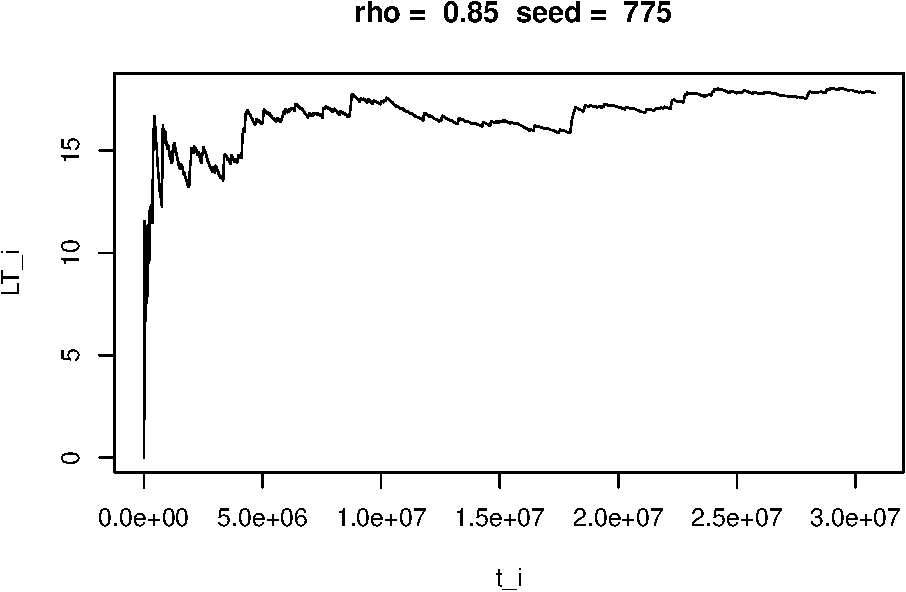
\includegraphics{003_files/figure-latex/unnamed-chunk-20-1.pdf}
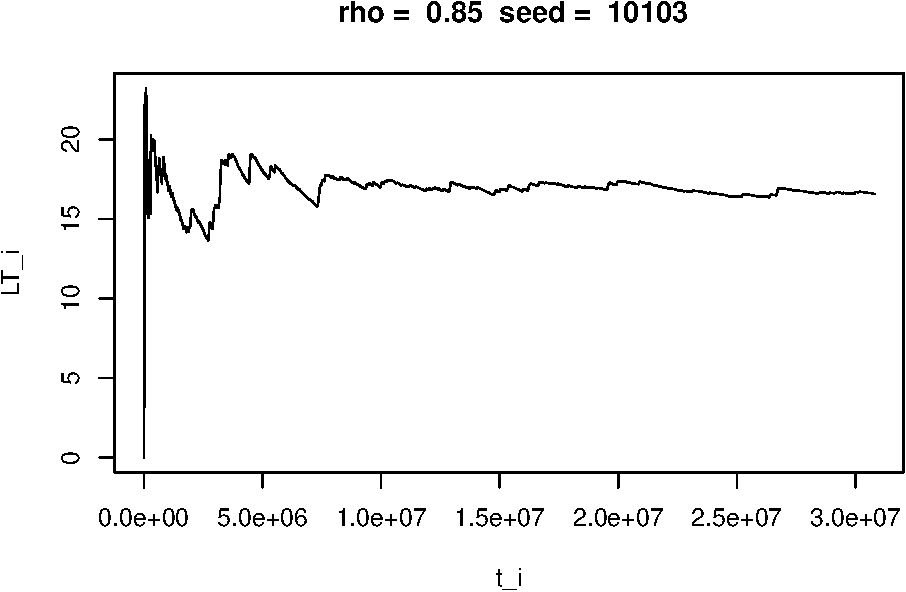
\includegraphics{003_files/figure-latex/unnamed-chunk-20-2.pdf}
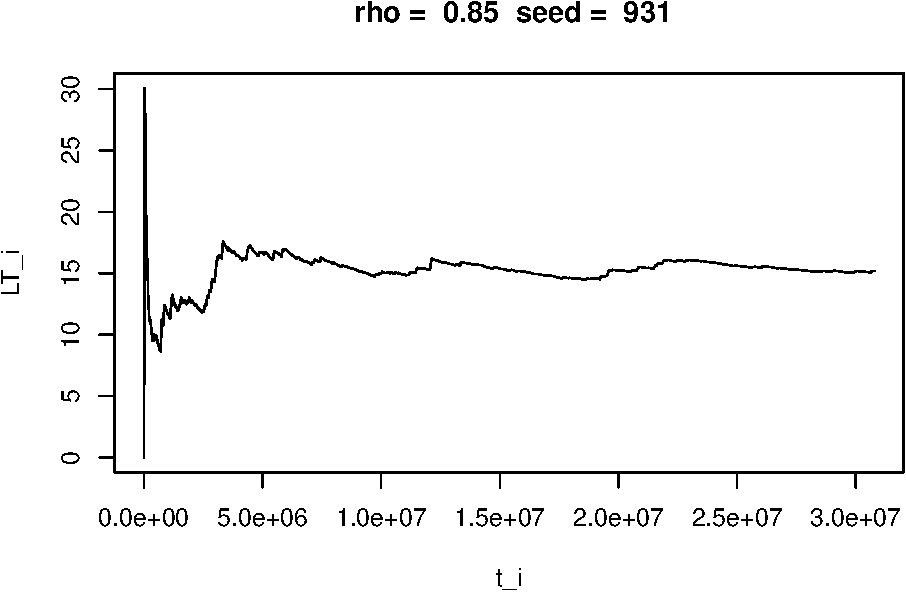
\includegraphics{003_files/figure-latex/unnamed-chunk-20-3.pdf}
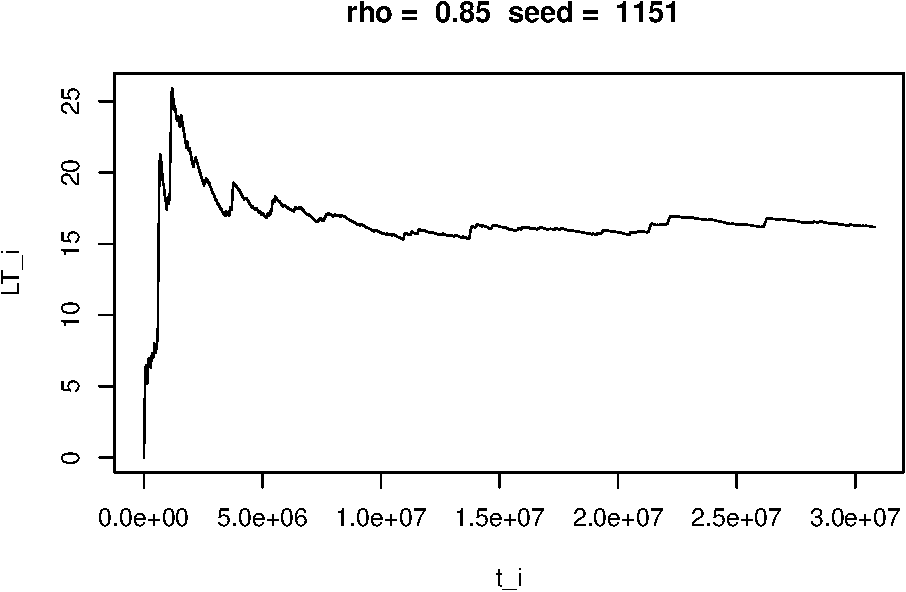
\includegraphics{003_files/figure-latex/unnamed-chunk-20-4.pdf}
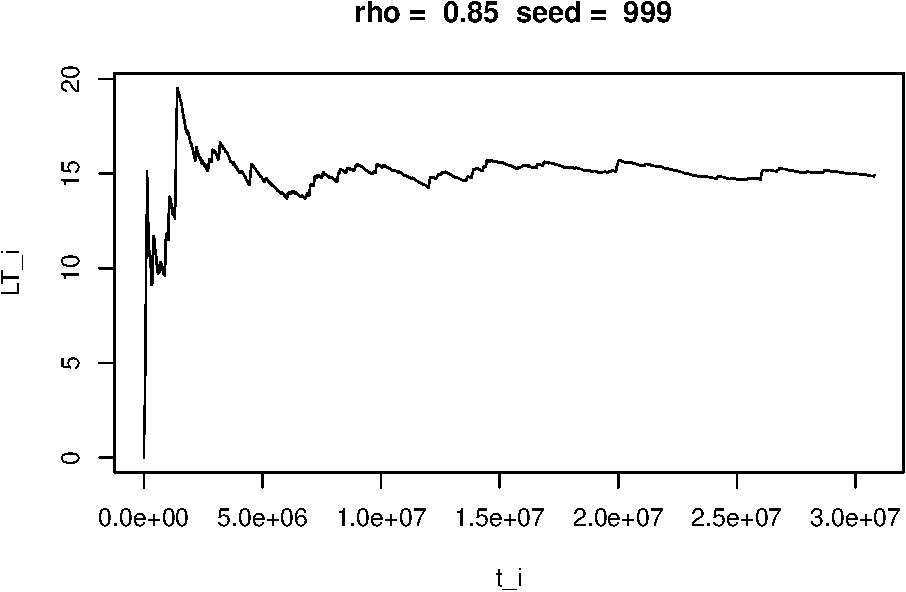
\includegraphics{003_files/figure-latex/unnamed-chunk-20-5.pdf}
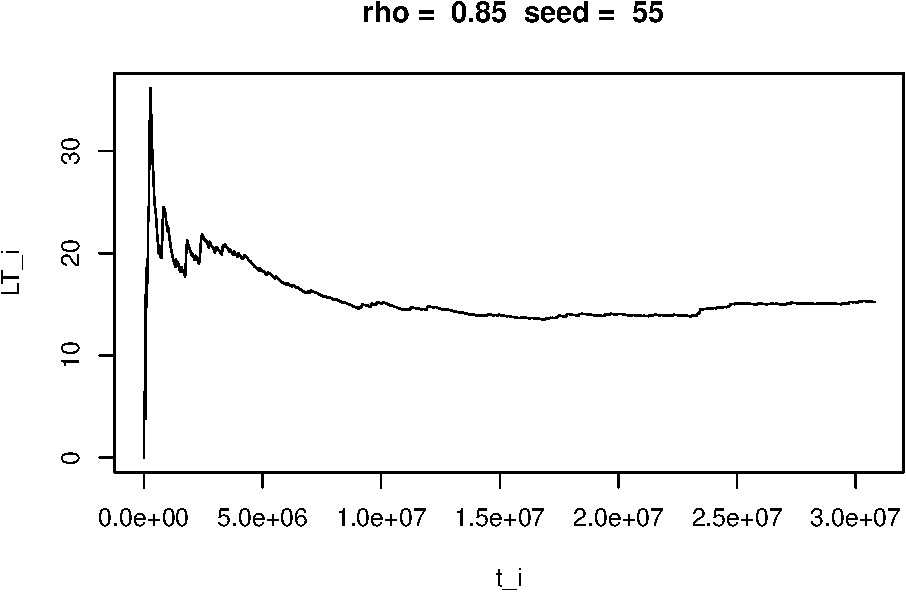
\includegraphics{003_files/figure-latex/unnamed-chunk-20-6.pdf}
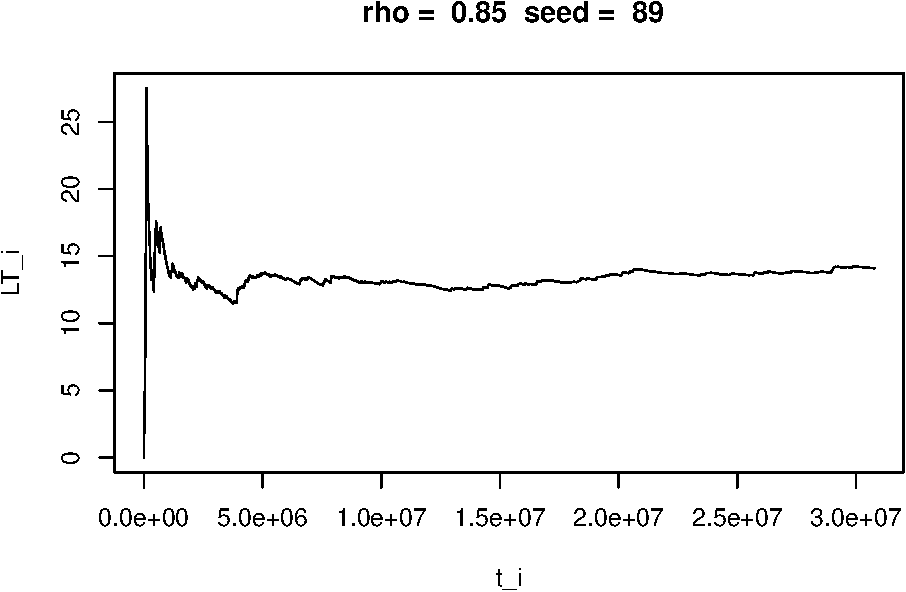
\includegraphics{003_files/figure-latex/unnamed-chunk-20-7.pdf}
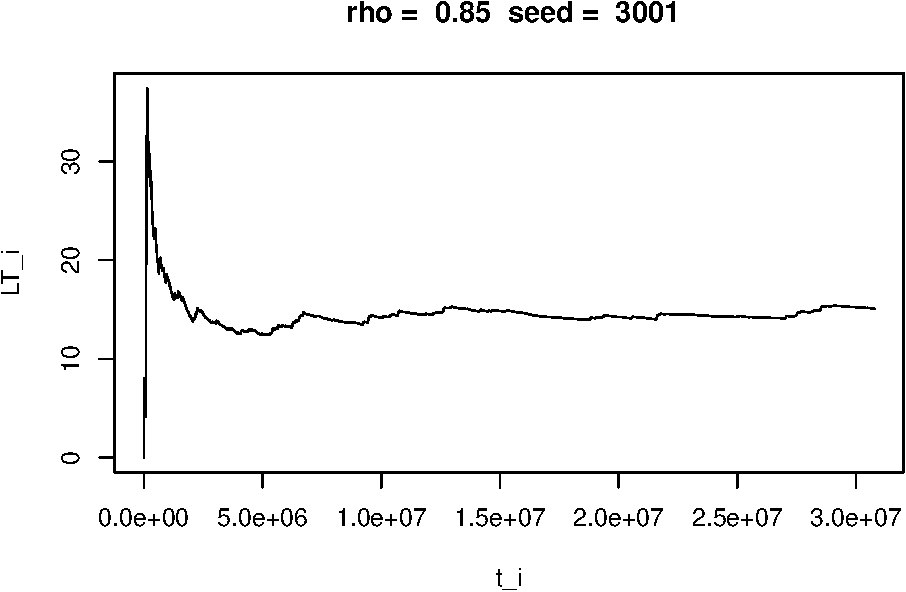
\includegraphics{003_files/figure-latex/unnamed-chunk-20-8.pdf}
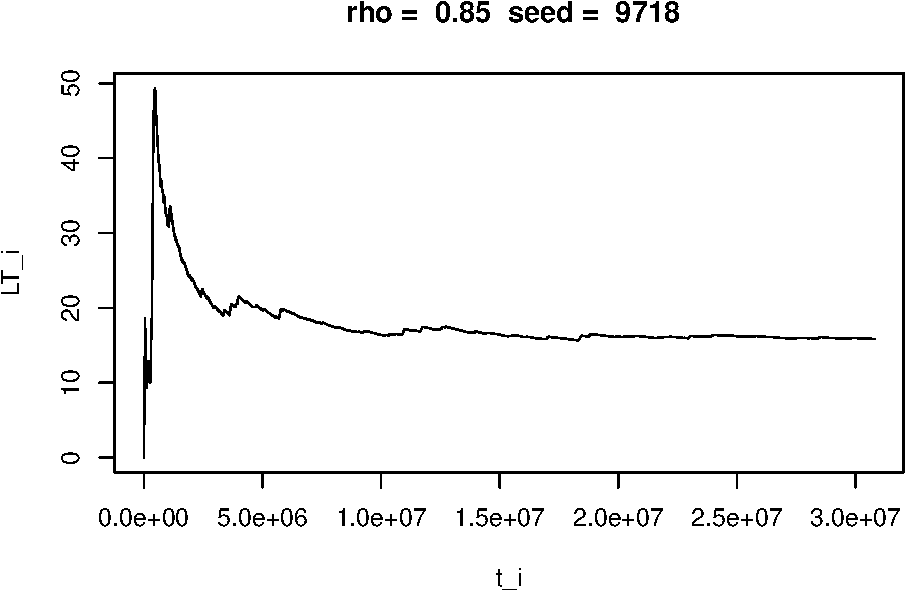
\includegraphics{003_files/figure-latex/unnamed-chunk-20-9.pdf}
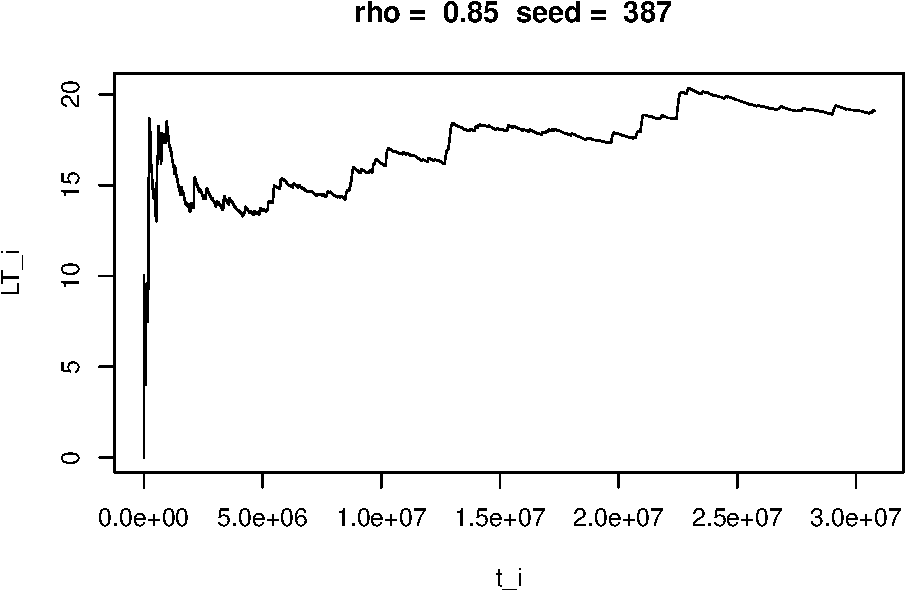
\includegraphics{003_files/figure-latex/unnamed-chunk-20-10.pdf}

We now compute the confidence interval for \(L_{q}\) and \(W_{q}\) using
the same procedure we detailed for \(\rho =\) 0.85. The computations
produce the followings confidence intervals for the average queue length
and waiting time:

\begin{longtable}[]{@{}llllll@{}}
\toprule
\(\rho\) & -C.I \(W_{q}\) & +C.I \(W_{q}\) & -C.I \(L_{q}\) & +C.I
\(L_{q}\) &\tabularnewline
\midrule
\endhead
0.85 & 14.2854646 & 16.016791 & 1099.7052017 &
1232.9696842\tabularnewline
\bottomrule
\end{longtable}

\subsubsection{\texorpdfstring{Loading factor \(\rho\) =
0.925}{Loading factor \textbackslash{}rho = 0.925}}\label{loading-factor-rho-0.925}

We generate 10 simulations with 100000 clients, each with a different
seed. We check if the steady state is attained. We also check for
irregularities in the simulation results, in which case we change the
random number generator seed and repeat the simulation.

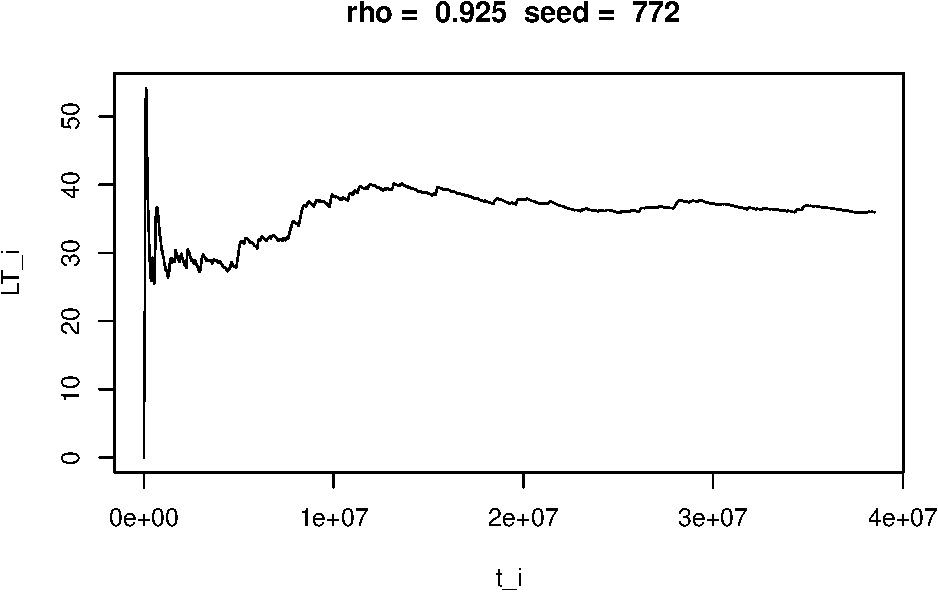
\includegraphics{003_files/figure-latex/unnamed-chunk-22-1.pdf}
\includegraphics{003_files/figure-latex/unnamed-chunk-22-2.pdf}
\includegraphics{003_files/figure-latex/unnamed-chunk-22-3.pdf}
\includegraphics{003_files/figure-latex/unnamed-chunk-22-4.pdf}
\includegraphics{003_files/figure-latex/unnamed-chunk-22-5.pdf}
\includegraphics{003_files/figure-latex/unnamed-chunk-22-6.pdf}
\includegraphics{003_files/figure-latex/unnamed-chunk-22-7.pdf}
\includegraphics{003_files/figure-latex/unnamed-chunk-22-8.pdf}
\includegraphics{003_files/figure-latex/unnamed-chunk-22-9.pdf}
\includegraphics{003_files/figure-latex/unnamed-chunk-22-10.pdf}

We now compute the confidence interval for \(L_{q}\) and \(W_{q}\) using
the same procedure we detailed for \(\rho =\) 0.925. The computations
produce the followings confidence intervals for the average queue length
and waiting time:

\begin{longtable}[]{@{}llllll@{}}
\toprule
\(\rho\) & -C.I \(W_{q}\) & +C.I \(W_{q}\) & -C.I \(L_{q}\) & +C.I
\(L_{q}\) &\tabularnewline
\midrule
\endhead
0.925 & 33.0165379 & 37.5147854 & 2542.0094174 &
2889.0200971\tabularnewline
\bottomrule
\end{longtable}

\subsection{Comparison of Allen Cuneen's approximation and the
simulation}\label{comparison-of-allen-cuneens-approximation-and-the-simulation}

\begin{longtable}[]{@{}llllllll@{}}
\toprule
\(\rho\) & \(W_{q}\) & -C.I \(W_{q}\) & +C.I \(W_{q}\) & \(L_{q}\) &
-C.I \(L_{q}\) & +C.I \(L_{q}\) &\tabularnewline
\midrule
\endhead
0.4 & 69.1507968 & 51.0353731 & 55.5687961 & 0.8980623 & 0.6629266 &
0.7216626\tabularnewline
0.7 & 423.5486306 & 379.3389492 & 412.4915102 & 5.5006316 & 4.9266678 &
5.3560657\tabularnewline
0.85 & 1249.0362678 & 1099.7052017 & 1232.9696842 & 16.2212502 &
14.2854646 & 16.016791\tabularnewline
0.925 & 2958.3575269 & 2542.0094174 & 2889.0200971 & 38.4202276 &
33.0165379 & 37.5147854\tabularnewline
\bottomrule
\end{longtable}

As we can see in the table above Allen-Cuneen's approximation values for
all loading factors are outside of the confidence interval of our
simulations, always above. Overall, the approximations of both, \(W_q\)
and \(L_{q}\), are not very far from the simulation's confidence
interval. So the Allen-Cuneen's aproximation models a system where the
occupancy is higher and the waiting times in the queue are also greater
than what our simulation produces. How can we explain that?

First of all, our random number generator has not been tested. As
discussed in class, it is impossible to generate real randomness, so
every rng must be tested for multiple desirable properties. In our
particular case, even though we used the rng that ships with R, which is
considered to ship with well tested generated random number streams, we
noticed that while repeatedly running the simulation we needed to change
the seed from time to time in order to avoid irregularities or abrupt
changes. We can conclude that we need to test the rng for appropriate
period, given that we need around 200.000 samples in each simulation.

Secondly, the Allen Cuneen's approximation uses the exact formula for
exponential models plus a correction factor. This correction factor may
not be accurate for the case. However, the Allen-Cuneen's aproximation
is said to be a good aproximation, usually with 5\% error or less. If we
compute the error of the Allen-Cuneen's aproximation formula in respect
to the mean of the confidence interval it is a bit greater than 5\%, but
close to it, except for the first loading factor \(\rho=0.4\). If we
compute the error of the aproximation formular in resptect to the upper
bound of the confidence interval it is less than 5\% except for the
first loading factor \(\rho=0.4\) (where it is bigger).

\begin{longtable}[]{@{}lllll@{}}
\toprule
& \(\rho=0.4\) & \(\rho=0.7\) & \(\rho=0.85\) &
\(\rho=0.925\)\tabularnewline
\midrule
\endhead
Error to the mean of the C.I. & -23\% & -7\% & -7\% &
-8\%\tabularnewline
Error to the upper bound of the C.I. & -20\% & -3\% & -1\% &
-2\%\tabularnewline
\bottomrule
\end{longtable}

Given that last comparison of relative errors, the aproximation seems
correct except for the first \(\rho=0.4\), where the error is too big to
be neglected. This may be caused by a Coefficient of deviation \(C_{x}\)
and a \(\sigma_{x}\) that are small, and that can affect significantly
the behaviour of the system, reducing the average occupancy. We see that
the expected value of the service times is close to 30 and that the
standard deviation is \(\sigma=1.4286\) so it can be considered small in
comparison with the expected value.

Finally, we may say that the last \(\rho=0.925\) could be high enough
that the theorem for ``heavy traffic'' conditions, the Köllerström
theorem, could be a better aproximation. It turns out this is not true.

\begin{longtable}[]{@{}llllllll@{}}
\toprule
\(\rho\) & \(W_{q}\) & -C.I \(W_{q}\) & +C.I \(W_{q}\) & \(L_{q}\) &
-C.I \(L_{q}\) & +C.I \(L_{q}\) &\tabularnewline
\midrule
\endhead
0.925 & 6.6689615 & 2542.0094174 & 2889.0200971 & 122.8694038 &
33.0165379 & 37.5147854\tabularnewline
\bottomrule
\end{longtable}

If we compute it, we can clearly see that it is a worse aproximation
than Allen Cuneen's formula. The reason is that 0.925 is not a close
value to 1, as is the requirement to consider a ``heavy loaded''
queueing system.


\end{document}
